\section{Standard algorithm}
Benchmarking the standard algorithm on the large set of problems provided earlier produced mixed results.
\Cref{tab:number-solved} lists the number of problems (out of the total number available from each set) that were solved by the in-the-middle algorithm.
The results indicate that the algorithm is able to solve the same types of problem as the \emph{Toulbar} and \emph{CPLEX} solvers, with a few exceptions.
This implies that the algorithm may be useful in most of the fields from which problems were drawn, but does not indicate whether it is useful in its current state, performance-wise.

However, as \cref{tab:comparative-results} shows, the algorithm performed very well when comparing runtime to other solvers and in fact it was the fastest for almost half of the sets after removing incomplete data (runtimes based on data where less than \SI{70}{\percent} of the problems were solved).
In most problem sets, the solution quality was good as well --- for several sets optimal solutions were found --- with the notable exception of the \emph{Scene Decomposition} set\footnote{Note however that the Toulbar2 solver finds the same non-optimal solutions in this problem set.}.

The algorithm shows promise especially in the Max-\gls{csp} and \gls{mrf} categories, where overall solution quality is good and the algorithm had the best performance for several sets.
Compared to both Toulbar2 and CPLEX, the in-the-middle algorithm appears to be a useful complement providing (good) approximative solutions to problems the other solvers have great difficulty in solving.
Results from the \gls{cp} category are also promising, but these problem sets are small and not all \gls{cp} problems have max-sum formulations.

\Cref{fig:cactus-std} shows accumulated runtimes for three of the sets in which the algorithm performed well.
The algorithm has a consistent advantage in the \emph{Segmentation} set (\cref{fig:cactus-std:segmentation}), which is reflected by the mean runtime in \cref{tab:comparative-results}.
\Cref{fig:cactus-std:blackhole,fig:cactus-std:dbn} highlight more interesting situations.
The former illustrates performance in the \emph{Black Hole} set and indicates a clear advantage in the second half of the set, which contains larger and more difficult problems.
% [fix] - the above says almost nothing. try to figure out why results are that way!

The latter instead shows an apparent advantage throughout the whole set, which is contradicted by \cref{tab:comparative-results}.
This has an explanation: while the in-the-middle algorithm has a lower runtime (by \SIrange{60}{80}{\percent}) for difficult problems, where Toulbar2 reaches the benchmark time limit, the situation is reversed for the less difficult problems where Toulbar2 is roughly \SI{99}{\percent} faster.
The bulk of the set consists of less difficult problems, which explains the median value.
% [todo] - justify choice of median for the values (goes in method?)

Analyzing the shortcomings of the algorithm, it is clear from \cref{tab:comparative-results} that it had significant difficulties in solving the problems from the \gls{cfn} category.
% large domains, large number of cost functions. memory issues? need background on toulbar first?
% most cost functions have arity 2, would better constraint update be useful?
% does cfn have a structure toulbar/cplex is using?

% [todo] - explain SceneDecomp anomaly? Maybe deGivry14 has something on it?

% [todo] - analyze which problems itm is bad at, an whether specialized updates may solve this

% Note: problems with many hard clauses are more efficiently solved by the implementation

% Mention: the omitted problems were omitted due to memory issues

% Note: scenedecomp very bad, but same solutions as toulbar2

% For conclusions?: note that a portfolio approach as suggested by deGivry14? may be beneficial, or rather that itm may be useful in such a portfolio

% [todo] - analyzing interesting problem sets
% [todo] - comparing with other solvers
% [todo] - identify what problems ITM is good at

% [review] - find a recent test of max-clique solvers on the WPMS-MaxClique set? (not for the table but may be interesting to refer rough timings) Östergård02 might be ok but that hardware is way too old.

\begin{table}
	\centering
	% Updated 2014-05-25
	\caption{
		Solution quality and runtime.
		For each problem instance used in the benchmark, the in-the-middle solver runtime is compared the other solvers included in the benchmark, and the objective value is compared to the best known optimum from \textcite{deGivry14}.
		%Problem sets marked with \textdagger{} include unsolved problems (no feasible solution found by the in-the-middle solver), and n/a values indicate that none of the problems in the set were solved.
		Runtimes based on less than \SI{70}{\percent} of the problems are faded, while the best runtime of those remaining is emphasised.
		%Some problem sets have been omitted.
	}
	% [review] - present in same way as deGivry14?
	% [todo] - double-check all table data!
	% [review] - including number solved may be interesting. additional table or appendix?
	\label{tab:comparative-results}
	\begin{figcenter}
	\begin{tabular}{xyHS[round-mode=places,round-precision=3,scientific-notation=fixed,fixed-exponent=0]
				    S[round-mode=places,round-precision=2,scientific-notation=fixed,fixed-exponent=0]
				    H%S[round-mode=places,round-precision=2,scientific-notation=fixed,fixed-exponent=0]
				    S[round-mode=places,round-precision=2,scientific-notation=fixed,fixed-exponent=0]
				    S[round-mode=places,round-precision=2,scientific-notation=fixed,fixed-exponent=0]
				    S[round-mode=places,round-precision=2,scientific-notation=fixed,fixed-exponent=0]}
		\toprule
			%{} & {} & \multicolumn{2}{c}{In-the-middle} & \multicolumn{5}{c}{Mean solution time (\si{\second})} \\
			%\cmidrule(rl){3-4} \cmidrule(rl){5-9}
			{} & {} & {} & {} & \multicolumn{5}{c}{Mean solution time (\si{\second})} \\
			\cmidrule(rl){5-9}
			{\normalsize Category} & {\normalsize Set} & {\(\#\) solved} & {Sol. diff. (\si{\percent})} & {ITM} & {MPLP2} & {Toulbar2} & {CPLEX} & {MaxHS} \\
		\midrule
\acrshort{cfn}	&	Auction\textdagger	&	{102/170}	&	0.000000e+00	&	\color{gray}82.8575	&	1200.00	&	8.195	&	\emshape 0.030	&	0.040 \\
				&	CELAR\textdagger	&	{10/16}	&	9.081260e-07	&	\color{gray}193.3445	&	1200.00	&	\emshape 22.375	&	1200.00	&	{\textcolor{gray}{n/a}} \\
				&	Pedigree	&	\emph{10/10}	&	1.804874e-00	&	\emshape 2.3750	&	{\textcolor{gray}{n/a}}	&	4.130	&	\color{gray}0.710	&	\color{gray}0.030 \\
				&	ProteinDesign	&	\emph{10/10}	&	0.000000e+00	&	43.3995	&	60.500	&	\emshape 2.330	&	1200.00	&	{\textcolor{gray}{n/a}} \\
				&	SPOT5\textdagger	&	{5/20}	&	4.977105e-03	&	\color{gray}6.4360	&	1200.00	&	1200.00	&	\emshape 0.465	&	\color{gray}0.820 \\
				&	Warehouse\textdagger	&	{38/55}	&	0.000000e+00	&	\color{gray}55.8550	&	57.970	&	0.160	&	\emshape 0.050	&	0.560 \\
%\acrshort{cp}	&	AMaze\textdagger	&	{0/6}	&	{\textcolor{gray}{n/a}}	&	{\textcolor{gray}{n/a}}	&	{\textcolor{gray}{n/a}}	&	544.545	&	{\textcolor{gray}{n/a}}	&	2.940 \\
%				&	FastFood\textdagger	&	{1/6}	&	0.000000e+00	&	0.0000	&	{\textcolor{gray}{n/a}}	&	0.0	&	0.010	&	0.0 \\
%\acrshort{cp}	&	Golomb\textdagger	&	{0/6}	&	{\textcolor{gray}{n/a}}	&	{\textcolor{gray}{n/a}}	&	{\textcolor{gray}{n/a}}	&	19.860	&	{\textcolor{gray}{n/a}}	&	42.670 \\
\acrshort{cp}	&	OnCallRostering\textdagger	&	{3/5}	&	4.000000e-06	&	\emshape 10.3540	&	{\textcolor{gray}{n/a}}	&	71.040	&	1200.0	&	18.950 \\
				&	ParityLearning	&	\emph{7/7}	&	1.800000e-05	&	\emshape 34.5300	&	{\textcolor{gray}{n/a}}	&	368.080	&	1200.0	&	\color{gray}222.690 \\
%				&	VRP\textdagger	&	{0/5}	&	{\textcolor{gray}{n/a}}	&	{\textcolor{gray}{n/a}}	&	{\textcolor{gray}{n/a}}	&	1200.0	&	{\textcolor{gray}{n/a}}	&	{\textcolor{gray}{n/a}} \\
%\acrshort{cvpr}	&	ChineseChars\textdagger	&	{0/100}	&	{\textcolor{gray}{n/a}}	&	{\textcolor{gray}{n/a}}	&	1200.00	&	1200.0	&	1200.0	&	{\textcolor{gray}{n/a}} \\
%				&	ColorSeg\textdagger	&	{0/21}	&	{\textcolor{gray}{n/a}}	&	{\textcolor{gray}{n/a}}	&	1200.00	&	1200.0	&	1200.0	&	{\textcolor{gray}{n/a}} \\
\acrshort{cvpr}	&	GeomSurf	&	\emph{600/600}	&	2.091307e-00	&	\emshape 0.0460	&	1.740	&	0.070	&	6.620	&	\color{gray}27.110 \\
				&	InPainting	&	\emph{4/4}	&	1.797097e-02	&	\emshape 1009.5145	&	1057.860	&	1200.0	&	1200.0	&	{\textcolor{gray}{n/a}} \\
				&	Matching	&	\emph{4/4}	&	0.000000e+00	&	17.9275	&	12.710	&	\emshape 4.120	&	1200.0	&	{\textcolor{gray}{n/a}} \\
%				&	MatchingStereo\textdagger	&	{0/2}	&	{\textcolor{gray}{n/a}}	&	{\textcolor{gray}{n/a}}	&	1200.00	&	1200.0	&	{\textcolor{gray}{n/a}}	&	{\textcolor{gray}{n/a}} \\
				&	ObjectSeg	&	\emph{5/5}	&	3.253700e-04	&	\emshape 1200.0	&	\emshape 1200.00	&	\emshape 1200.0	&	\emshape 1200.0	&	{\textcolor{gray}{n/a}} \\
%				&	PhotoMontage\textdagger	&	{0/2}	&	{\textcolor{gray}{n/a}}	&	{\textcolor{gray}{n/a}}	&	{\textcolor{gray}{n/a}}	&	{\textcolor{gray}{n/a}}	&	{\textcolor{gray}{n/a}}	&	{\textcolor{gray}{n/a}} \\
				&	SceneDecomp	&	\emph{715/715}	&	7.545481e+01	&	0.0210	&	0.110	&	\emshape 0.020	&	1200.0	&	\color{gray}521.160 \\
Max-\acrshort{csp}	&	BlackHole	&	\emph{37/37}	&	9.009009e-01	&	\emshape 58.8900	&	{\textcolor{gray}{n/a}}	&	1200.0	&	315.050	&	\color{gray}0.635 \\
				&	Coloring	&	\emph{22/22}	&	0.000000e+00	&	1.6860	&	{\textcolor{gray}{n/a}}	&	\emshape 0.405	&	1.275	&	\color{gray}0.030 \\
				&	Composed	&	\emph{80/80}	&	1.342282e-01	&	20.3400	&	1200.00	&	\emshape 0.115	&	5.755	&	32.690 \\
				&	EHI	&	{200/200}	&	9.000000e-01	&	\emshape 191.2190	&	{\textcolor{gray}{n/a}}	&	1200.0	&	1200.0	&	{\textcolor{gray}{n/a}} \\
				&	Geometric	&	\emph{100/100}	&	1.082434e-00	&	98.9760	&	{\textcolor{gray}{n/a}}	&	0.620	&	1200.0	&	\emshape 0.150 \\
				&	Langford	&	\emph{4/4}	&	1.311265e-00	&	\emshape 70.7775	&	1200.00	&	600.255	&	851.605	&	\color{gray}0.270 \\
				&	QCP	&	\emph{60/60}	&	1.292034e-00	&	43.2575	&	1200.00	&	1200.0	&	1200.0	&	\emshape 0.125 \\
\acrshort{mrf}	&	DBN	&	\emph{108/108}	&	0.000000e+00	&	37.9040	&	1200.00	&	\emshape 0.180	&	48.280	&	\color{gray}20.020 \\
				&	Grid\textdagger	&	{0/21}	&	{\textcolor{gray}{n/a}}	&	{\textcolor{gray}{n/a}}	&	1200.00	&	1200.0	&	\emshape 160.640	&	\color{gray}542.850 \\
				&	ImageAlignment	&	\emph{10/10}	&	0.000000e+00	&	\emshape 0.5815	&	4.855	&	1.800	&	1200.0	&	{\textcolor{gray}{n/a}} \\
				&	Linkage\textdagger	&	{8/22}	&	0.000000e+00	&	\color{gray}41.0700	&	1200.00	&	32.050	&	327.625	&	\emshape 16.520 \\
				&	ObjectDetection	&	\emph{37/37}	&	6.465565e-00	&	\emshape 279.8620	&	1200.00	&	1200.0	&	1200.0	&	{\textcolor{gray}{n/a}} \\
				&	ProteinFolding\textdagger	&	{20/21}	&	0.000000e+00	&	1200.0000	&	1200.00	&	\emshape 23.140	&	\color{gray}116.735	&	{\textcolor{gray}{n/a}} \\
				&	Segmentation	&	\emph{100/100}	&	0.000000e+00	&	\emshape 0.0310	&	0.355	&	0.150	&	600.070	&	\color{gray}0.300 \\
%\acrshort{wpms}	&	Haplotyping	&	{0/100}	&	{\textcolor{gray}{n/a}}	&	{\textcolor{gray}{n/a}}	&	{\textcolor{gray}{n/a}}	&	1200.0	&	1200.0	&	5.200 \\
\acrshort{wpms}	&	MaxClique\textdagger	&	{46/62}	&	2.583333e-00	&	\emshape 257.0920	&	1200.00	&	389.745	&	481.550	&	\color{gray}8.795 \\
%				&	MIPLib\textdagger	&	{0/12}	&	{\textcolor{gray}{n/a}}	&	{\textcolor{gray}{n/a}}	&	{\textcolor{gray}{n/a}}	&	193.990	&	533.220	&	0.360 \\
%				&	PackupWeighted\textdagger	&	{0/99}	&	{\textcolor{gray}{n/a}}	&	{\textcolor{gray}{n/a}}	&	{\textcolor{gray}{n/a}}	&	292.960	&	0.280	&	4.620 \\
%				&	PlanningWithPref	&	{0/29}	&	{\textcolor{gray}{n/a}}	&	{\textcolor{gray}{n/a}}	&	{\textcolor{gray}{n/a}}	&	1200.0	&	1200.0	&	1.270 \\
%				&	TimeTabling	&	{0/25}	&	{\textcolor{gray}{n/a}}	&	{\textcolor{gray}{n/a}}	&	{\textcolor{gray}{n/a}}	&	1200.0	&	1200.0	&	83.800 \\
%				&	Upgradeability\textdagger	&	{0/100}	&	{\textcolor{gray}{n/a}}	&	{\textcolor{gray}{n/a}}	&	{\textcolor{gray}{n/a}}	&	3.095	&	1.010	&	24.985 \\
		\bottomrule
	\end{tabular}
	\end{figcenter}
\end{table}

\begin{figure}
	\begin{figcenter}
	\subfloat[The \emph{Black Hole} set of the Max-\gls{csp} category.\label{fig:cactus-std:blackhole}]{% Created by tikzDevice version 0.7.0 on 2014-06-01 21:53:23
% !TEX encoding = UTF-8 Unicode
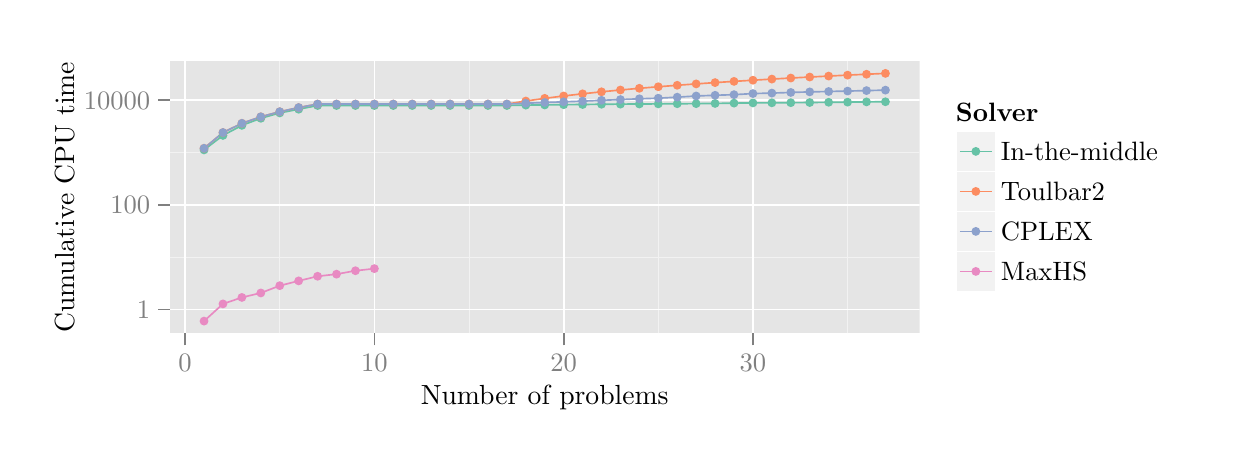
\begin{tikzpicture}[x=1pt,y=1pt]
\definecolor[named]{fillColor}{rgb}{1.00,1.00,1.00}
\path[use as bounding box,fill=fillColor,fill opacity=0.00] (0,0) rectangle (433.62,144.54);
\begin{scope}
\path[clip] (  0.00,  0.00) rectangle (433.62,144.54);
\definecolor[named]{drawColor}{rgb}{1.00,1.00,1.00}
\definecolor[named]{fillColor}{rgb}{1.00,1.00,1.00}

\path[draw=drawColor,line width= 0.6pt,line join=round,line cap=round,fill=fillColor] (  0.00,  0.00) rectangle (433.62,144.54);
\end{scope}
\begin{scope}
\path[clip] ( 51.42, 34.03) rectangle (322.26,132.50);
\definecolor[named]{fillColor}{rgb}{0.90,0.90,0.90}

\path[fill=fillColor] ( 51.42, 34.03) rectangle (322.26,132.50);
\definecolor[named]{drawColor}{rgb}{0.95,0.95,0.95}

\path[draw=drawColor,line width= 0.3pt,line join=round] ( 51.42, 61.62) --
	(322.26, 61.62);

\path[draw=drawColor,line width= 0.3pt,line join=round] ( 51.42, 99.45) --
	(322.26, 99.45);

\path[draw=drawColor,line width= 0.3pt,line join=round] ( 91.09, 34.03) --
	( 91.09,132.50);

\path[draw=drawColor,line width= 0.3pt,line join=round] (159.48, 34.03) --
	(159.48,132.50);

\path[draw=drawColor,line width= 0.3pt,line join=round] (227.87, 34.03) --
	(227.87,132.50);

\path[draw=drawColor,line width= 0.3pt,line join=round] (296.27, 34.03) --
	(296.27,132.50);
\definecolor[named]{drawColor}{rgb}{1.00,1.00,1.00}

\path[draw=drawColor,line width= 0.6pt,line join=round] ( 51.42, 42.71) --
	(322.26, 42.71);

\path[draw=drawColor,line width= 0.6pt,line join=round] ( 51.42, 80.53) --
	(322.26, 80.53);

\path[draw=drawColor,line width= 0.6pt,line join=round] ( 51.42,118.36) --
	(322.26,118.36);

\path[draw=drawColor,line width= 0.6pt,line join=round] ( 56.89, 34.03) --
	( 56.89,132.50);

\path[draw=drawColor,line width= 0.6pt,line join=round] (125.28, 34.03) --
	(125.28,132.50);

\path[draw=drawColor,line width= 0.6pt,line join=round] (193.68, 34.03) --
	(193.68,132.50);

\path[draw=drawColor,line width= 0.6pt,line join=round] (262.07, 34.03) --
	(262.07,132.50);
\definecolor[named]{drawColor}{rgb}{0.40,0.76,0.65}

\path[draw=drawColor,line width= 0.6pt,line join=round] ( 63.73,100.37) --
	( 70.57,105.60) --
	( 77.41,109.24) --
	( 84.25,111.79) --
	( 91.09,113.73) --
	( 97.92,115.07) --
	(104.76,116.41) --
	(111.60,116.41) --
	(118.44,116.41) --
	(125.28,116.41) --
	(132.12,116.41) --
	(138.96,116.41) --
	(145.80,116.41) --
	(152.64,116.41) --
	(159.48,116.41) --
	(166.32,116.41) --
	(173.16,116.41) --
	(180.00,116.55) --
	(186.84,116.61) --
	(193.68,116.71) --
	(200.52,116.77) --
	(207.35,116.87) --
	(214.19,116.91) --
	(221.03,116.96) --
	(227.87,117.00) --
	(234.71,117.06) --
	(241.55,117.09) --
	(248.39,117.16) --
	(255.23,117.27) --
	(262.07,117.35) --
	(268.91,117.38) --
	(275.75,117.43) --
	(282.59,117.49) --
	(289.43,117.58) --
	(296.27,117.63) --
	(303.11,117.72) --
	(309.95,117.77);
\definecolor[named]{drawColor}{rgb}{0.99,0.55,0.38}

\path[draw=drawColor,line width= 0.6pt,line join=round] ( 63.73,100.95) --
	( 70.57,106.64) --
	( 77.41,109.97) --
	( 84.25,112.33) --
	( 91.09,114.17) --
	( 97.92,115.66) --
	(104.76,116.93) --
	(111.60,116.93) --
	(118.44,116.93) --
	(125.28,116.93) --
	(132.12,116.93) --
	(138.96,116.93) --
	(145.80,116.93) --
	(152.64,116.93) --
	(159.48,116.93) --
	(166.32,116.93) --
	(173.16,116.93) --
	(180.00,118.03) --
	(186.84,119.00) --
	(193.68,119.86) --
	(200.52,120.64) --
	(207.35,121.36) --
	(214.19,122.02) --
	(221.03,122.63) --
	(227.87,123.19) --
	(234.71,123.72) --
	(241.55,124.22) --
	(248.39,124.69) --
	(255.23,125.13) --
	(262.07,125.55) --
	(268.91,125.96) --
	(275.75,126.34) --
	(282.59,126.70) --
	(289.43,127.05) --
	(296.27,127.39) --
	(303.11,127.71) --
	(309.95,128.02);
\definecolor[named]{drawColor}{rgb}{0.55,0.63,0.80}

\path[draw=drawColor,line width= 0.6pt,line join=round] ( 63.73,100.95) --
	( 70.57,106.64) --
	( 77.41,109.97) --
	( 84.25,112.33) --
	( 91.09,114.17) --
	( 97.92,115.66) --
	(104.76,116.93) --
	(111.60,116.93) --
	(118.44,116.93) --
	(125.28,116.93) --
	(132.12,116.93) --
	(138.96,116.93) --
	(145.80,116.93) --
	(152.64,116.93) --
	(159.48,116.93) --
	(166.32,116.93) --
	(173.16,116.93) --
	(180.00,117.24) --
	(186.84,117.50) --
	(193.68,117.74) --
	(200.52,117.99) --
	(207.35,118.29) --
	(214.19,118.56) --
	(221.03,118.84) --
	(227.87,119.06) --
	(234.71,119.43) --
	(241.55,119.85) --
	(248.39,120.11) --
	(255.23,120.33) --
	(262.07,120.73) --
	(268.91,120.90) --
	(275.75,121.13) --
	(282.59,121.33) --
	(289.43,121.48) --
	(296.27,121.63) --
	(303.11,121.80) --
	(309.95,121.97);
\definecolor[named]{drawColor}{rgb}{0.91,0.54,0.76}

\path[draw=drawColor,line width= 0.6pt,line join=round] ( 63.73, 38.51) --
	( 70.57, 44.73) --
	( 77.41, 47.06) --
	( 84.25, 48.68) --
	( 91.09, 51.31) --
	( 97.92, 53.04) --
	(104.76, 54.71) --
	(111.60, 55.47) --
	(118.44, 56.71) --
	(125.28, 57.47);
\definecolor[named]{fillColor}{rgb}{0.40,0.76,0.65}

\path[fill=fillColor] ( 63.73,100.37) circle (  1.60);

\path[fill=fillColor] ( 70.57,105.60) circle (  1.60);

\path[fill=fillColor] ( 77.41,109.24) circle (  1.60);

\path[fill=fillColor] ( 84.25,111.79) circle (  1.60);

\path[fill=fillColor] ( 91.09,113.73) circle (  1.60);

\path[fill=fillColor] ( 97.92,115.07) circle (  1.60);

\path[fill=fillColor] (104.76,116.41) circle (  1.60);

\path[fill=fillColor] (111.60,116.41) circle (  1.60);

\path[fill=fillColor] (118.44,116.41) circle (  1.60);

\path[fill=fillColor] (125.28,116.41) circle (  1.60);

\path[fill=fillColor] (132.12,116.41) circle (  1.60);

\path[fill=fillColor] (138.96,116.41) circle (  1.60);

\path[fill=fillColor] (145.80,116.41) circle (  1.60);

\path[fill=fillColor] (152.64,116.41) circle (  1.60);

\path[fill=fillColor] (159.48,116.41) circle (  1.60);

\path[fill=fillColor] (166.32,116.41) circle (  1.60);

\path[fill=fillColor] (173.16,116.41) circle (  1.60);

\path[fill=fillColor] (180.00,116.55) circle (  1.60);

\path[fill=fillColor] (186.84,116.61) circle (  1.60);

\path[fill=fillColor] (193.68,116.71) circle (  1.60);

\path[fill=fillColor] (200.52,116.77) circle (  1.60);

\path[fill=fillColor] (207.35,116.87) circle (  1.60);

\path[fill=fillColor] (214.19,116.91) circle (  1.60);

\path[fill=fillColor] (221.03,116.96) circle (  1.60);

\path[fill=fillColor] (227.87,117.00) circle (  1.60);

\path[fill=fillColor] (234.71,117.06) circle (  1.60);

\path[fill=fillColor] (241.55,117.09) circle (  1.60);

\path[fill=fillColor] (248.39,117.16) circle (  1.60);

\path[fill=fillColor] (255.23,117.27) circle (  1.60);

\path[fill=fillColor] (262.07,117.35) circle (  1.60);

\path[fill=fillColor] (268.91,117.38) circle (  1.60);

\path[fill=fillColor] (275.75,117.43) circle (  1.60);

\path[fill=fillColor] (282.59,117.49) circle (  1.60);

\path[fill=fillColor] (289.43,117.58) circle (  1.60);

\path[fill=fillColor] (296.27,117.63) circle (  1.60);

\path[fill=fillColor] (303.11,117.72) circle (  1.60);

\path[fill=fillColor] (309.95,117.77) circle (  1.60);
\definecolor[named]{fillColor}{rgb}{0.99,0.55,0.38}

\path[fill=fillColor] ( 63.73,100.95) circle (  1.60);

\path[fill=fillColor] ( 70.57,106.64) circle (  1.60);

\path[fill=fillColor] ( 77.41,109.97) circle (  1.60);

\path[fill=fillColor] ( 84.25,112.33) circle (  1.60);

\path[fill=fillColor] ( 91.09,114.17) circle (  1.60);

\path[fill=fillColor] ( 97.92,115.66) circle (  1.60);

\path[fill=fillColor] (104.76,116.93) circle (  1.60);

\path[fill=fillColor] (111.60,116.93) circle (  1.60);

\path[fill=fillColor] (118.44,116.93) circle (  1.60);

\path[fill=fillColor] (125.28,116.93) circle (  1.60);

\path[fill=fillColor] (132.12,116.93) circle (  1.60);

\path[fill=fillColor] (138.96,116.93) circle (  1.60);

\path[fill=fillColor] (145.80,116.93) circle (  1.60);

\path[fill=fillColor] (152.64,116.93) circle (  1.60);

\path[fill=fillColor] (159.48,116.93) circle (  1.60);

\path[fill=fillColor] (166.32,116.93) circle (  1.60);

\path[fill=fillColor] (173.16,116.93) circle (  1.60);

\path[fill=fillColor] (180.00,118.03) circle (  1.60);

\path[fill=fillColor] (186.84,119.00) circle (  1.60);

\path[fill=fillColor] (193.68,119.86) circle (  1.60);

\path[fill=fillColor] (200.52,120.64) circle (  1.60);

\path[fill=fillColor] (207.35,121.36) circle (  1.60);

\path[fill=fillColor] (214.19,122.02) circle (  1.60);

\path[fill=fillColor] (221.03,122.63) circle (  1.60);

\path[fill=fillColor] (227.87,123.19) circle (  1.60);

\path[fill=fillColor] (234.71,123.72) circle (  1.60);

\path[fill=fillColor] (241.55,124.22) circle (  1.60);

\path[fill=fillColor] (248.39,124.69) circle (  1.60);

\path[fill=fillColor] (255.23,125.13) circle (  1.60);

\path[fill=fillColor] (262.07,125.55) circle (  1.60);

\path[fill=fillColor] (268.91,125.96) circle (  1.60);

\path[fill=fillColor] (275.75,126.34) circle (  1.60);

\path[fill=fillColor] (282.59,126.70) circle (  1.60);

\path[fill=fillColor] (289.43,127.05) circle (  1.60);

\path[fill=fillColor] (296.27,127.39) circle (  1.60);

\path[fill=fillColor] (303.11,127.71) circle (  1.60);

\path[fill=fillColor] (309.95,128.02) circle (  1.60);
\definecolor[named]{fillColor}{rgb}{0.55,0.63,0.80}

\path[fill=fillColor] ( 63.73,100.95) circle (  1.60);

\path[fill=fillColor] ( 70.57,106.64) circle (  1.60);

\path[fill=fillColor] ( 77.41,109.97) circle (  1.60);

\path[fill=fillColor] ( 84.25,112.33) circle (  1.60);

\path[fill=fillColor] ( 91.09,114.17) circle (  1.60);

\path[fill=fillColor] ( 97.92,115.66) circle (  1.60);

\path[fill=fillColor] (104.76,116.93) circle (  1.60);

\path[fill=fillColor] (111.60,116.93) circle (  1.60);

\path[fill=fillColor] (118.44,116.93) circle (  1.60);

\path[fill=fillColor] (125.28,116.93) circle (  1.60);

\path[fill=fillColor] (132.12,116.93) circle (  1.60);

\path[fill=fillColor] (138.96,116.93) circle (  1.60);

\path[fill=fillColor] (145.80,116.93) circle (  1.60);

\path[fill=fillColor] (152.64,116.93) circle (  1.60);

\path[fill=fillColor] (159.48,116.93) circle (  1.60);

\path[fill=fillColor] (166.32,116.93) circle (  1.60);

\path[fill=fillColor] (173.16,116.93) circle (  1.60);

\path[fill=fillColor] (180.00,117.24) circle (  1.60);

\path[fill=fillColor] (186.84,117.50) circle (  1.60);

\path[fill=fillColor] (193.68,117.74) circle (  1.60);

\path[fill=fillColor] (200.52,117.99) circle (  1.60);

\path[fill=fillColor] (207.35,118.29) circle (  1.60);

\path[fill=fillColor] (214.19,118.56) circle (  1.60);

\path[fill=fillColor] (221.03,118.84) circle (  1.60);

\path[fill=fillColor] (227.87,119.06) circle (  1.60);

\path[fill=fillColor] (234.71,119.43) circle (  1.60);

\path[fill=fillColor] (241.55,119.85) circle (  1.60);

\path[fill=fillColor] (248.39,120.11) circle (  1.60);

\path[fill=fillColor] (255.23,120.33) circle (  1.60);

\path[fill=fillColor] (262.07,120.73) circle (  1.60);

\path[fill=fillColor] (268.91,120.90) circle (  1.60);

\path[fill=fillColor] (275.75,121.13) circle (  1.60);

\path[fill=fillColor] (282.59,121.33) circle (  1.60);

\path[fill=fillColor] (289.43,121.48) circle (  1.60);

\path[fill=fillColor] (296.27,121.63) circle (  1.60);

\path[fill=fillColor] (303.11,121.80) circle (  1.60);

\path[fill=fillColor] (309.95,121.97) circle (  1.60);
\definecolor[named]{fillColor}{rgb}{0.91,0.54,0.76}

\path[fill=fillColor] ( 63.73, 38.51) circle (  1.60);

\path[fill=fillColor] ( 70.57, 44.73) circle (  1.60);

\path[fill=fillColor] ( 77.41, 47.06) circle (  1.60);

\path[fill=fillColor] ( 84.25, 48.68) circle (  1.60);

\path[fill=fillColor] ( 91.09, 51.31) circle (  1.60);

\path[fill=fillColor] ( 97.92, 53.04) circle (  1.60);

\path[fill=fillColor] (104.76, 54.71) circle (  1.60);

\path[fill=fillColor] (111.60, 55.47) circle (  1.60);

\path[fill=fillColor] (118.44, 56.71) circle (  1.60);

\path[fill=fillColor] (125.28, 57.47) circle (  1.60);
\end{scope}
\begin{scope}
\path[clip] (  0.00,  0.00) rectangle (433.62,144.54);
\definecolor[named]{drawColor}{rgb}{0.50,0.50,0.50}

\node[text=drawColor,anchor=base east,inner sep=0pt, outer sep=0pt, scale=  0.96] at ( 44.30, 39.40) {1};

\node[text=drawColor,anchor=base east,inner sep=0pt, outer sep=0pt, scale=  0.96] at ( 44.30, 77.23) {100};

\node[text=drawColor,anchor=base east,inner sep=0pt, outer sep=0pt, scale=  0.96] at ( 44.30,115.06) {10000};
\end{scope}
\begin{scope}
\path[clip] (  0.00,  0.00) rectangle (433.62,144.54);
\definecolor[named]{drawColor}{rgb}{0.50,0.50,0.50}

\path[draw=drawColor,line width= 0.6pt,line join=round] ( 47.15, 42.71) --
	( 51.42, 42.71);

\path[draw=drawColor,line width= 0.6pt,line join=round] ( 47.15, 80.53) --
	( 51.42, 80.53);

\path[draw=drawColor,line width= 0.6pt,line join=round] ( 47.15,118.36) --
	( 51.42,118.36);
\end{scope}
\begin{scope}
\path[clip] (  0.00,  0.00) rectangle (433.62,144.54);
\definecolor[named]{drawColor}{rgb}{0.50,0.50,0.50}

\path[draw=drawColor,line width= 0.6pt,line join=round] ( 56.89, 29.77) --
	( 56.89, 34.03);

\path[draw=drawColor,line width= 0.6pt,line join=round] (125.28, 29.77) --
	(125.28, 34.03);

\path[draw=drawColor,line width= 0.6pt,line join=round] (193.68, 29.77) --
	(193.68, 34.03);

\path[draw=drawColor,line width= 0.6pt,line join=round] (262.07, 29.77) --
	(262.07, 34.03);
\end{scope}
\begin{scope}
\path[clip] (  0.00,  0.00) rectangle (433.62,144.54);
\definecolor[named]{drawColor}{rgb}{0.50,0.50,0.50}

\node[text=drawColor,anchor=base,inner sep=0pt, outer sep=0pt, scale=  0.96] at ( 56.89, 20.31) {0};

\node[text=drawColor,anchor=base,inner sep=0pt, outer sep=0pt, scale=  0.96] at (125.28, 20.31) {10};

\node[text=drawColor,anchor=base,inner sep=0pt, outer sep=0pt, scale=  0.96] at (193.68, 20.31) {20};

\node[text=drawColor,anchor=base,inner sep=0pt, outer sep=0pt, scale=  0.96] at (262.07, 20.31) {30};
\end{scope}
\begin{scope}
\path[clip] (  0.00,  0.00) rectangle (433.62,144.54);
\definecolor[named]{drawColor}{rgb}{0.00,0.00,0.00}

\node[text=drawColor,anchor=base,inner sep=0pt, outer sep=0pt, scale=  1] at (186.84,  8.53) {Number of problems};
\end{scope}
\begin{scope}
\path[clip] (  0.00,  0.00) rectangle (433.62,144.54);
\definecolor[named]{drawColor}{rgb}{0.00,0.00,0.00}

\node[text=drawColor,rotate= 90.00,anchor=base,inner sep=0pt, outer sep=0pt, scale=  1] at ( 16.80, 83.26) {Cumulative CPU time};
\end{scope}
\begin{scope}
\path[clip] (  0.00,  0.00) rectangle (433.62,144.54);
\definecolor[named]{fillColor}{rgb}{1.00,1.00,1.00}

\path[fill=fillColor] (331.12, 44.97) rectangle (412.71,121.56);
\end{scope}
\begin{scope}
\path[clip] (  0.00,  0.00) rectangle (433.62,144.54);
\definecolor[named]{drawColor}{rgb}{0.00,0.00,0.00}

\node[text=drawColor,anchor=base west,inner sep=0pt, outer sep=0pt, scale=  0.96] at (335.39,110.67) {\bfseries Solver};
\end{scope}
\begin{scope}
\path[clip] (  0.00,  0.00) rectangle (433.62,144.54);
\definecolor[named]{drawColor}{rgb}{1.00,1.00,1.00}
\definecolor[named]{fillColor}{rgb}{0.95,0.95,0.95}

\path[draw=drawColor,line width= 0.6pt,line join=round,line cap=round,fill=fillColor] (335.39, 92.60) rectangle (349.85,107.05);
\end{scope}
\begin{scope}
\path[clip] (  0.00,  0.00) rectangle (433.62,144.54);
\definecolor[named]{drawColor}{rgb}{0.40,0.76,0.65}

\path[draw=drawColor,line width= 0.6pt,line join=round] (336.84, 99.83) -- (348.40, 99.83);
\end{scope}
\begin{scope}
\path[clip] (  0.00,  0.00) rectangle (433.62,144.54);
\definecolor[named]{fillColor}{rgb}{0.40,0.76,0.65}

\path[fill=fillColor] (342.62, 99.83) circle (  1.60);
\end{scope}
\begin{scope}
\path[clip] (  0.00,  0.00) rectangle (433.62,144.54);
\definecolor[named]{drawColor}{rgb}{1.00,1.00,1.00}
\definecolor[named]{fillColor}{rgb}{0.95,0.95,0.95}

\path[draw=drawColor,line width= 0.6pt,line join=round,line cap=round,fill=fillColor] (335.39, 78.15) rectangle (349.85, 92.60);
\end{scope}
\begin{scope}
\path[clip] (  0.00,  0.00) rectangle (433.62,144.54);
\definecolor[named]{drawColor}{rgb}{0.99,0.55,0.38}

\path[draw=drawColor,line width= 0.6pt,line join=round] (336.84, 85.37) -- (348.40, 85.37);
\end{scope}
\begin{scope}
\path[clip] (  0.00,  0.00) rectangle (433.62,144.54);
\definecolor[named]{fillColor}{rgb}{0.99,0.55,0.38}

\path[fill=fillColor] (342.62, 85.37) circle (  1.60);
\end{scope}
\begin{scope}
\path[clip] (  0.00,  0.00) rectangle (433.62,144.54);
\definecolor[named]{drawColor}{rgb}{1.00,1.00,1.00}
\definecolor[named]{fillColor}{rgb}{0.95,0.95,0.95}

\path[draw=drawColor,line width= 0.6pt,line join=round,line cap=round,fill=fillColor] (335.39, 63.69) rectangle (349.85, 78.15);
\end{scope}
\begin{scope}
\path[clip] (  0.00,  0.00) rectangle (433.62,144.54);
\definecolor[named]{drawColor}{rgb}{0.55,0.63,0.80}

\path[draw=drawColor,line width= 0.6pt,line join=round] (336.84, 70.92) -- (348.40, 70.92);
\end{scope}
\begin{scope}
\path[clip] (  0.00,  0.00) rectangle (433.62,144.54);
\definecolor[named]{fillColor}{rgb}{0.55,0.63,0.80}

\path[fill=fillColor] (342.62, 70.92) circle (  1.60);
\end{scope}
\begin{scope}
\path[clip] (  0.00,  0.00) rectangle (433.62,144.54);
\definecolor[named]{drawColor}{rgb}{1.00,1.00,1.00}
\definecolor[named]{fillColor}{rgb}{0.95,0.95,0.95}

\path[draw=drawColor,line width= 0.6pt,line join=round,line cap=round,fill=fillColor] (335.39, 49.24) rectangle (349.85, 63.69);
\end{scope}
\begin{scope}
\path[clip] (  0.00,  0.00) rectangle (433.62,144.54);
\definecolor[named]{drawColor}{rgb}{0.91,0.54,0.76}

\path[draw=drawColor,line width= 0.6pt,line join=round] (336.84, 56.46) -- (348.40, 56.46);
\end{scope}
\begin{scope}
\path[clip] (  0.00,  0.00) rectangle (433.62,144.54);
\definecolor[named]{fillColor}{rgb}{0.91,0.54,0.76}

\path[fill=fillColor] (342.62, 56.46) circle (  1.60);
\end{scope}
\begin{scope}
\path[clip] (  0.00,  0.00) rectangle (433.62,144.54);
\definecolor[named]{drawColor}{rgb}{0.00,0.00,0.00}

\node[text=drawColor,anchor=base west,inner sep=0pt, outer sep=0pt, scale=  0.96] at (351.65, 96.52) {In-the-middle};
\end{scope}
\begin{scope}
\path[clip] (  0.00,  0.00) rectangle (433.62,144.54);
\definecolor[named]{drawColor}{rgb}{0.00,0.00,0.00}

\node[text=drawColor,anchor=base west,inner sep=0pt, outer sep=0pt, scale=  0.96] at (351.65, 82.07) {Toulbar2};
\end{scope}
\begin{scope}
\path[clip] (  0.00,  0.00) rectangle (433.62,144.54);
\definecolor[named]{drawColor}{rgb}{0.00,0.00,0.00}

\node[text=drawColor,anchor=base west,inner sep=0pt, outer sep=0pt, scale=  0.96] at (351.65, 67.61) {CPLEX};
\end{scope}
\begin{scope}
\path[clip] (  0.00,  0.00) rectangle (433.62,144.54);
\definecolor[named]{drawColor}{rgb}{0.00,0.00,0.00}

\node[text=drawColor,anchor=base west,inner sep=0pt, outer sep=0pt, scale=  0.96] at (351.65, 53.16) {MaxHS};
\end{scope}
\end{tikzpicture}
}
	\end{figcenter}
	\\
	\begin{figcenter}
	\subfloat[The \emph{DBN} set of the \gls{mrf} category.\label{fig:cactus-std:dbn}]{% Created by tikzDevice version 0.7.0 on 2014-06-05 13:06:24
% !TEX encoding = UTF-8 Unicode
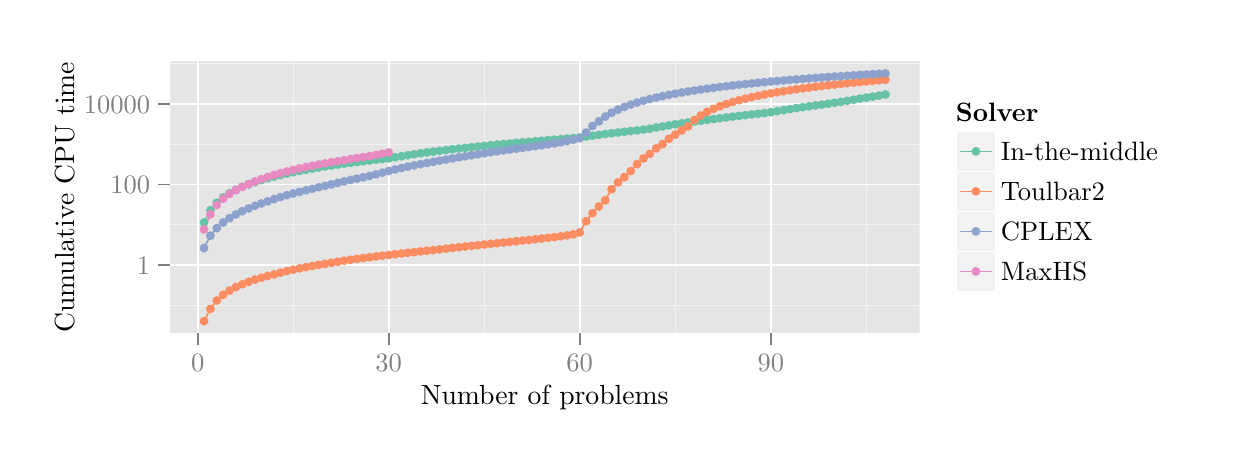
\begin{tikzpicture}[x=1pt,y=1pt]
\definecolor[named]{fillColor}{rgb}{1.00,1.00,1.00}
\path[use as bounding box,fill=fillColor,fill opacity=0.00] (0,0) rectangle (433.62,144.54);
\begin{scope}
\path[clip] (  0.00,  0.00) rectangle (433.62,144.54);
\definecolor[named]{drawColor}{rgb}{1.00,1.00,1.00}
\definecolor[named]{fillColor}{rgb}{1.00,1.00,1.00}

\path[draw=drawColor,line width= 0.6pt,line join=round,line cap=round,fill=fillColor] (  0.00,  0.00) rectangle (433.62,144.54);
\end{scope}
\begin{scope}
\path[clip] ( 51.42, 34.03) rectangle (322.26,132.50);
\definecolor[named]{fillColor}{rgb}{0.90,0.90,0.90}

\path[fill=fillColor] ( 51.42, 34.03) rectangle (322.26,132.50);
\definecolor[named]{drawColor}{rgb}{0.95,0.95,0.95}

\path[draw=drawColor,line width= 0.3pt,line join=round] ( 51.42, 44.29) --
	(322.26, 44.29);

\path[draw=drawColor,line width= 0.3pt,line join=round] ( 51.42, 73.36) --
	(322.26, 73.36);

\path[draw=drawColor,line width= 0.3pt,line join=round] ( 51.42,102.43) --
	(322.26,102.43);

\path[draw=drawColor,line width= 0.3pt,line join=round] ( 51.42,131.49) --
	(322.26,131.49);

\path[draw=drawColor,line width= 0.3pt,line join=round] ( 95.94, 34.03) --
	( 95.94,132.50);

\path[draw=drawColor,line width= 0.3pt,line join=round] (164.98, 34.03) --
	(164.98,132.50);

\path[draw=drawColor,line width= 0.3pt,line join=round] (234.01, 34.03) --
	(234.01,132.50);

\path[draw=drawColor,line width= 0.3pt,line join=round] (303.04, 34.03) --
	(303.04,132.50);
\definecolor[named]{drawColor}{rgb}{1.00,1.00,1.00}

\path[draw=drawColor,line width= 0.6pt,line join=round] ( 51.42, 58.83) --
	(322.26, 58.83);

\path[draw=drawColor,line width= 0.6pt,line join=round] ( 51.42, 87.89) --
	(322.26, 87.89);

\path[draw=drawColor,line width= 0.6pt,line join=round] ( 51.42,116.96) --
	(322.26,116.96);

\path[draw=drawColor,line width= 0.6pt,line join=round] ( 61.43, 34.03) --
	( 61.43,132.50);

\path[draw=drawColor,line width= 0.6pt,line join=round] (130.46, 34.03) --
	(130.46,132.50);

\path[draw=drawColor,line width= 0.6pt,line join=round] (199.49, 34.03) --
	(199.49,132.50);

\path[draw=drawColor,line width= 0.6pt,line join=round] (268.53, 34.03) --
	(268.53,132.50);
\definecolor[named]{drawColor}{rgb}{0.40,0.76,0.65}

\path[draw=drawColor,line width= 0.6pt,line join=round] ( 63.73, 74.14) --
	( 66.03, 78.58) --
	( 68.33, 81.30) --
	( 70.63, 83.21) --
	( 72.93, 84.72) --
	( 75.23, 85.96) --
	( 77.53, 87.01) --
	( 79.84, 87.91) --
	( 82.14, 88.70) --
	( 84.44, 89.45) --
	( 86.74, 90.12) --
	( 89.04, 90.74) --
	( 91.34, 91.30) --
	( 93.64, 91.82) --
	( 95.94, 92.31) --
	( 98.24, 92.77) --
	(100.55, 93.20) --
	(102.85, 93.61) --
	(105.15, 94.00) --
	(107.45, 94.37) --
	(109.75, 94.73) --
	(112.05, 95.06) --
	(114.35, 95.39) --
	(116.65, 95.69) --
	(118.95, 95.99) --
	(121.26, 96.27) --
	(123.56, 96.54) --
	(125.86, 96.81) --
	(128.16, 97.06) --
	(130.46, 97.32) --
	(132.76, 97.71) --
	(135.06, 98.09) --
	(137.36, 98.45) --
	(139.66, 98.79) --
	(141.97, 99.13) --
	(144.27, 99.44) --
	(146.57, 99.75) --
	(148.87,100.04) --
	(151.17,100.32) --
	(153.47,100.59) --
	(155.77,100.85) --
	(158.07,101.10) --
	(160.37,101.35) --
	(162.68,101.59) --
	(164.98,101.82) --
	(167.28,102.05) --
	(169.58,102.27) --
	(171.88,102.48) --
	(174.18,102.69) --
	(176.48,102.90) --
	(178.78,103.10) --
	(181.08,103.31) --
	(183.39,103.51) --
	(185.69,103.71) --
	(187.99,103.90) --
	(190.29,104.09) --
	(192.59,104.27) --
	(194.89,104.45) --
	(197.19,104.65) --
	(199.49,104.84) --
	(201.79,105.18) --
	(204.09,105.50) --
	(206.40,105.81) --
	(208.70,106.11) --
	(211.00,106.39) --
	(213.30,106.66) --
	(215.60,106.92) --
	(217.90,107.18) --
	(220.20,107.42) --
	(222.50,107.71) --
	(224.80,108.02) --
	(227.11,108.45) --
	(229.41,108.85) --
	(231.71,109.24) --
	(234.01,109.61) --
	(236.31,109.96) --
	(238.61,110.30) --
	(240.91,110.62) --
	(243.21,110.93) --
	(245.51,111.23) --
	(247.82,111.53) --
	(250.12,111.82) --
	(252.42,112.09) --
	(254.72,112.38) --
	(257.02,112.66) --
	(259.32,112.92) --
	(261.62,113.18) --
	(263.92,113.44) --
	(266.22,113.69) --
	(268.53,113.98) --
	(270.83,114.38) --
	(273.13,114.74) --
	(275.43,115.11) --
	(277.73,115.46) --
	(280.03,115.79) --
	(282.33,116.11) --
	(284.63,116.43) --
	(286.93,116.75) --
	(289.24,117.07) --
	(291.54,117.40) --
	(293.84,117.73) --
	(296.14,118.13) --
	(298.44,118.51) --
	(300.74,118.89) --
	(303.04,119.25) --
	(305.34,119.62) --
	(307.64,119.98) --
	(309.95,120.40);
\definecolor[named]{drawColor}{rgb}{0.99,0.55,0.38}

\path[draw=drawColor,line width= 0.6pt,line join=round] ( 63.73, 38.51) --
	( 66.03, 42.89) --
	( 68.33, 45.95) --
	( 70.63, 48.00) --
	( 72.93, 49.55) --
	( 75.23, 50.79) --
	( 77.53, 51.83) --
	( 79.84, 52.72) --
	( 82.14, 53.50) --
	( 84.44, 54.19) --
	( 86.74, 54.82) --
	( 89.04, 55.39) --
	( 91.34, 56.01) --
	( 93.64, 56.58) --
	( 95.94, 57.09) --
	( 98.24, 57.57) --
	(100.55, 58.02) --
	(102.85, 58.44) --
	(105.15, 58.83) --
	(107.45, 59.19) --
	(109.75, 59.60) --
	(112.05, 59.98) --
	(114.35, 60.34) --
	(116.65, 60.67) --
	(118.95, 61.00) --
	(121.26, 61.30) --
	(123.56, 61.59) --
	(125.86, 61.87) --
	(128.16, 62.14) --
	(130.46, 62.40) --
	(132.76, 62.68) --
	(135.06, 62.94) --
	(137.36, 63.20) --
	(139.66, 63.45) --
	(141.97, 63.69) --
	(144.27, 63.92) --
	(146.57, 64.17) --
	(148.87, 64.43) --
	(151.17, 64.69) --
	(153.47, 64.95) --
	(155.77, 65.21) --
	(158.07, 65.46) --
	(160.37, 65.70) --
	(162.68, 65.95) --
	(164.98, 66.19) --
	(167.28, 66.42) --
	(169.58, 66.66) --
	(171.88, 66.89) --
	(174.18, 67.14) --
	(176.48, 67.37) --
	(178.78, 67.61) --
	(181.08, 67.85) --
	(183.39, 68.09) --
	(185.69, 68.35) --
	(187.99, 68.60) --
	(190.29, 68.85) --
	(192.59, 69.15) --
	(194.89, 69.49) --
	(197.19, 69.85) --
	(199.49, 70.52) --
	(201.79, 74.59) --
	(204.09, 77.50) --
	(206.40, 79.91) --
	(208.70, 82.12) --
	(211.00, 86.15) --
	(213.30, 88.63) --
	(215.60, 90.53) --
	(217.90, 92.73) --
	(220.20, 95.24) --
	(222.50, 97.27) --
	(224.80, 98.95) --
	(227.11,100.92) --
	(229.41,102.44) --
	(231.71,104.38) --
	(234.01,105.88) --
	(236.31,107.39) --
	(238.61,108.88) --
	(240.91,111.15) --
	(243.21,112.81) --
	(245.51,114.12) --
	(247.82,115.21) --
	(250.12,116.14) --
	(252.42,116.95) --
	(254.72,117.67) --
	(257.02,118.31) --
	(259.32,118.89) --
	(261.62,119.43) --
	(263.92,119.92) --
	(266.22,120.38) --
	(268.53,120.80) --
	(270.83,121.20) --
	(273.13,121.58) --
	(275.43,121.93) --
	(277.73,122.27) --
	(280.03,122.59) --
	(282.33,122.89) --
	(284.63,123.18) --
	(286.93,123.46) --
	(289.24,123.72) --
	(291.54,123.97) --
	(293.84,124.22) --
	(296.14,124.45) --
	(298.44,124.68) --
	(300.74,124.90) --
	(303.04,125.11) --
	(305.34,125.32) --
	(307.64,125.52) --
	(309.95,125.71);
\definecolor[named]{drawColor}{rgb}{0.55,0.63,0.80}

\path[draw=drawColor,line width= 0.6pt,line join=round] ( 63.73, 64.91) --
	( 66.03, 69.35) --
	( 68.33, 72.09) --
	( 70.63, 74.15) --
	( 72.93, 75.71) --
	( 75.23, 77.03) --
	( 77.53, 78.21) --
	( 79.84, 79.22) --
	( 82.14, 80.17) --
	( 84.44, 81.02) --
	( 86.74, 81.80) --
	( 89.04, 82.58) --
	( 91.34, 83.32) --
	( 93.64, 83.99) --
	( 95.94, 84.63) --
	( 98.24, 85.21) --
	(100.55, 85.78) --
	(102.85, 86.31) --
	(105.15, 86.87) --
	(107.45, 87.38) --
	(109.75, 87.88) --
	(112.05, 88.47) --
	(114.35, 89.01) --
	(116.65, 89.51) --
	(118.95, 89.99) --
	(121.26, 90.46) --
	(123.56, 90.98) --
	(125.86, 91.53) --
	(128.16, 92.16) --
	(130.46, 92.75) --
	(132.76, 93.30) --
	(135.06, 93.82) --
	(137.36, 94.31) --
	(139.66, 94.78) --
	(141.97, 95.22) --
	(144.27, 95.64) --
	(146.57, 96.06) --
	(148.87, 96.47) --
	(151.17, 96.87) --
	(153.47, 97.29) --
	(155.77, 97.69) --
	(158.07, 98.07) --
	(160.37, 98.43) --
	(162.68, 98.80) --
	(164.98, 99.16) --
	(167.28, 99.51) --
	(169.58, 99.84) --
	(171.88,100.17) --
	(174.18,100.48) --
	(176.48,100.79) --
	(178.78,101.09) --
	(181.08,101.40) --
	(183.39,101.71) --
	(185.69,102.01) --
	(187.99,102.36) --
	(190.29,102.70) --
	(192.59,103.11) --
	(194.89,103.56) --
	(197.19,104.07) --
	(199.49,104.59) --
	(201.79,106.63) --
	(204.09,109.00) --
	(206.40,110.73) --
	(208.70,112.41) --
	(211.00,113.80) --
	(213.30,114.94) --
	(215.60,115.91) --
	(217.90,116.74) --
	(220.20,117.48) --
	(222.50,118.14) --
	(224.80,118.74) --
	(227.11,119.29) --
	(229.41,119.79) --
	(231.71,120.26) --
	(234.01,120.69) --
	(236.31,121.10) --
	(238.61,121.48) --
	(240.91,121.84) --
	(243.21,122.18) --
	(245.51,122.50) --
	(247.82,122.81) --
	(250.12,123.10) --
	(252.42,123.38) --
	(254.72,123.65) --
	(257.02,123.91) --
	(259.32,124.16) --
	(261.62,124.39) --
	(263.92,124.62) --
	(266.22,124.84) --
	(268.53,125.06) --
	(270.83,125.26) --
	(273.13,125.46) --
	(275.43,125.66) --
	(277.73,125.85) --
	(280.03,126.03) --
	(282.33,126.21) --
	(284.63,126.38) --
	(286.93,126.55) --
	(289.24,126.71) --
	(291.54,126.87) --
	(293.84,127.03) --
	(296.14,127.18) --
	(298.44,127.33) --
	(300.74,127.47) --
	(303.04,127.61) --
	(305.34,127.75) --
	(307.64,127.89) --
	(309.95,128.02);
\definecolor[named]{drawColor}{rgb}{0.91,0.54,0.76}

\path[draw=drawColor,line width= 0.6pt,line join=round] ( 63.73, 71.65) --
	( 66.03, 77.07) --
	( 68.33, 80.43) --
	( 70.63, 82.72) --
	( 72.93, 84.46) --
	( 75.23, 85.86) --
	( 77.53, 87.01) --
	( 79.84, 88.00) --
	( 82.14, 88.95) --
	( 84.44, 89.82) --
	( 86.74, 90.61) --
	( 89.04, 91.32) --
	( 91.34, 91.97) --
	( 93.64, 92.58) --
	( 95.94, 93.13) --
	( 98.24, 93.68) --
	(100.55, 94.18) --
	(102.85, 94.65) --
	(105.15, 95.09) --
	(107.45, 95.52) --
	(109.75, 95.92) --
	(112.05, 96.31) --
	(114.35, 96.69) --
	(116.65, 97.06) --
	(118.95, 97.43) --
	(121.26, 97.80) --
	(123.56, 98.16) --
	(125.86, 98.57) --
	(128.16, 99.01) --
	(130.46, 99.47);
\definecolor[named]{fillColor}{rgb}{0.40,0.76,0.65}

\path[fill=fillColor] ( 63.73, 74.14) circle (  1.60);

\path[fill=fillColor] ( 66.03, 78.58) circle (  1.60);

\path[fill=fillColor] ( 68.33, 81.30) circle (  1.60);

\path[fill=fillColor] ( 70.63, 83.21) circle (  1.60);

\path[fill=fillColor] ( 72.93, 84.72) circle (  1.60);

\path[fill=fillColor] ( 75.23, 85.96) circle (  1.60);

\path[fill=fillColor] ( 77.53, 87.01) circle (  1.60);

\path[fill=fillColor] ( 79.84, 87.91) circle (  1.60);

\path[fill=fillColor] ( 82.14, 88.70) circle (  1.60);

\path[fill=fillColor] ( 84.44, 89.45) circle (  1.60);

\path[fill=fillColor] ( 86.74, 90.12) circle (  1.60);

\path[fill=fillColor] ( 89.04, 90.74) circle (  1.60);

\path[fill=fillColor] ( 91.34, 91.30) circle (  1.60);

\path[fill=fillColor] ( 93.64, 91.82) circle (  1.60);

\path[fill=fillColor] ( 95.94, 92.31) circle (  1.60);

\path[fill=fillColor] ( 98.24, 92.77) circle (  1.60);

\path[fill=fillColor] (100.55, 93.20) circle (  1.60);

\path[fill=fillColor] (102.85, 93.61) circle (  1.60);

\path[fill=fillColor] (105.15, 94.00) circle (  1.60);

\path[fill=fillColor] (107.45, 94.37) circle (  1.60);

\path[fill=fillColor] (109.75, 94.73) circle (  1.60);

\path[fill=fillColor] (112.05, 95.06) circle (  1.60);

\path[fill=fillColor] (114.35, 95.39) circle (  1.60);

\path[fill=fillColor] (116.65, 95.69) circle (  1.60);

\path[fill=fillColor] (118.95, 95.99) circle (  1.60);

\path[fill=fillColor] (121.26, 96.27) circle (  1.60);

\path[fill=fillColor] (123.56, 96.54) circle (  1.60);

\path[fill=fillColor] (125.86, 96.81) circle (  1.60);

\path[fill=fillColor] (128.16, 97.06) circle (  1.60);

\path[fill=fillColor] (130.46, 97.32) circle (  1.60);

\path[fill=fillColor] (132.76, 97.71) circle (  1.60);

\path[fill=fillColor] (135.06, 98.09) circle (  1.60);

\path[fill=fillColor] (137.36, 98.45) circle (  1.60);

\path[fill=fillColor] (139.66, 98.79) circle (  1.60);

\path[fill=fillColor] (141.97, 99.13) circle (  1.60);

\path[fill=fillColor] (144.27, 99.44) circle (  1.60);

\path[fill=fillColor] (146.57, 99.75) circle (  1.60);

\path[fill=fillColor] (148.87,100.04) circle (  1.60);

\path[fill=fillColor] (151.17,100.32) circle (  1.60);

\path[fill=fillColor] (153.47,100.59) circle (  1.60);

\path[fill=fillColor] (155.77,100.85) circle (  1.60);

\path[fill=fillColor] (158.07,101.10) circle (  1.60);

\path[fill=fillColor] (160.37,101.35) circle (  1.60);

\path[fill=fillColor] (162.68,101.59) circle (  1.60);

\path[fill=fillColor] (164.98,101.82) circle (  1.60);

\path[fill=fillColor] (167.28,102.05) circle (  1.60);

\path[fill=fillColor] (169.58,102.27) circle (  1.60);

\path[fill=fillColor] (171.88,102.48) circle (  1.60);

\path[fill=fillColor] (174.18,102.69) circle (  1.60);

\path[fill=fillColor] (176.48,102.90) circle (  1.60);

\path[fill=fillColor] (178.78,103.10) circle (  1.60);

\path[fill=fillColor] (181.08,103.31) circle (  1.60);

\path[fill=fillColor] (183.39,103.51) circle (  1.60);

\path[fill=fillColor] (185.69,103.71) circle (  1.60);

\path[fill=fillColor] (187.99,103.90) circle (  1.60);

\path[fill=fillColor] (190.29,104.09) circle (  1.60);

\path[fill=fillColor] (192.59,104.27) circle (  1.60);

\path[fill=fillColor] (194.89,104.45) circle (  1.60);

\path[fill=fillColor] (197.19,104.65) circle (  1.60);

\path[fill=fillColor] (199.49,104.84) circle (  1.60);

\path[fill=fillColor] (201.79,105.18) circle (  1.60);

\path[fill=fillColor] (204.09,105.50) circle (  1.60);

\path[fill=fillColor] (206.40,105.81) circle (  1.60);

\path[fill=fillColor] (208.70,106.11) circle (  1.60);

\path[fill=fillColor] (211.00,106.39) circle (  1.60);

\path[fill=fillColor] (213.30,106.66) circle (  1.60);

\path[fill=fillColor] (215.60,106.92) circle (  1.60);

\path[fill=fillColor] (217.90,107.18) circle (  1.60);

\path[fill=fillColor] (220.20,107.42) circle (  1.60);

\path[fill=fillColor] (222.50,107.71) circle (  1.60);

\path[fill=fillColor] (224.80,108.02) circle (  1.60);

\path[fill=fillColor] (227.11,108.45) circle (  1.60);

\path[fill=fillColor] (229.41,108.85) circle (  1.60);

\path[fill=fillColor] (231.71,109.24) circle (  1.60);

\path[fill=fillColor] (234.01,109.61) circle (  1.60);

\path[fill=fillColor] (236.31,109.96) circle (  1.60);

\path[fill=fillColor] (238.61,110.30) circle (  1.60);

\path[fill=fillColor] (240.91,110.62) circle (  1.60);

\path[fill=fillColor] (243.21,110.93) circle (  1.60);

\path[fill=fillColor] (245.51,111.23) circle (  1.60);

\path[fill=fillColor] (247.82,111.53) circle (  1.60);

\path[fill=fillColor] (250.12,111.82) circle (  1.60);

\path[fill=fillColor] (252.42,112.09) circle (  1.60);

\path[fill=fillColor] (254.72,112.38) circle (  1.60);

\path[fill=fillColor] (257.02,112.66) circle (  1.60);

\path[fill=fillColor] (259.32,112.92) circle (  1.60);

\path[fill=fillColor] (261.62,113.18) circle (  1.60);

\path[fill=fillColor] (263.92,113.44) circle (  1.60);

\path[fill=fillColor] (266.22,113.69) circle (  1.60);

\path[fill=fillColor] (268.53,113.98) circle (  1.60);

\path[fill=fillColor] (270.83,114.38) circle (  1.60);

\path[fill=fillColor] (273.13,114.74) circle (  1.60);

\path[fill=fillColor] (275.43,115.11) circle (  1.60);

\path[fill=fillColor] (277.73,115.46) circle (  1.60);

\path[fill=fillColor] (280.03,115.79) circle (  1.60);

\path[fill=fillColor] (282.33,116.11) circle (  1.60);

\path[fill=fillColor] (284.63,116.43) circle (  1.60);

\path[fill=fillColor] (286.93,116.75) circle (  1.60);

\path[fill=fillColor] (289.24,117.07) circle (  1.60);

\path[fill=fillColor] (291.54,117.40) circle (  1.60);

\path[fill=fillColor] (293.84,117.73) circle (  1.60);

\path[fill=fillColor] (296.14,118.13) circle (  1.60);

\path[fill=fillColor] (298.44,118.51) circle (  1.60);

\path[fill=fillColor] (300.74,118.89) circle (  1.60);

\path[fill=fillColor] (303.04,119.25) circle (  1.60);

\path[fill=fillColor] (305.34,119.62) circle (  1.60);

\path[fill=fillColor] (307.64,119.98) circle (  1.60);

\path[fill=fillColor] (309.95,120.40) circle (  1.60);
\definecolor[named]{fillColor}{rgb}{0.99,0.55,0.38}

\path[fill=fillColor] ( 63.73, 38.51) circle (  1.60);

\path[fill=fillColor] ( 66.03, 42.89) circle (  1.60);

\path[fill=fillColor] ( 68.33, 45.95) circle (  1.60);

\path[fill=fillColor] ( 70.63, 48.00) circle (  1.60);

\path[fill=fillColor] ( 72.93, 49.55) circle (  1.60);

\path[fill=fillColor] ( 75.23, 50.79) circle (  1.60);

\path[fill=fillColor] ( 77.53, 51.83) circle (  1.60);

\path[fill=fillColor] ( 79.84, 52.72) circle (  1.60);

\path[fill=fillColor] ( 82.14, 53.50) circle (  1.60);

\path[fill=fillColor] ( 84.44, 54.19) circle (  1.60);

\path[fill=fillColor] ( 86.74, 54.82) circle (  1.60);

\path[fill=fillColor] ( 89.04, 55.39) circle (  1.60);

\path[fill=fillColor] ( 91.34, 56.01) circle (  1.60);

\path[fill=fillColor] ( 93.64, 56.58) circle (  1.60);

\path[fill=fillColor] ( 95.94, 57.09) circle (  1.60);

\path[fill=fillColor] ( 98.24, 57.57) circle (  1.60);

\path[fill=fillColor] (100.55, 58.02) circle (  1.60);

\path[fill=fillColor] (102.85, 58.44) circle (  1.60);

\path[fill=fillColor] (105.15, 58.83) circle (  1.60);

\path[fill=fillColor] (107.45, 59.19) circle (  1.60);

\path[fill=fillColor] (109.75, 59.60) circle (  1.60);

\path[fill=fillColor] (112.05, 59.98) circle (  1.60);

\path[fill=fillColor] (114.35, 60.34) circle (  1.60);

\path[fill=fillColor] (116.65, 60.67) circle (  1.60);

\path[fill=fillColor] (118.95, 61.00) circle (  1.60);

\path[fill=fillColor] (121.26, 61.30) circle (  1.60);

\path[fill=fillColor] (123.56, 61.59) circle (  1.60);

\path[fill=fillColor] (125.86, 61.87) circle (  1.60);

\path[fill=fillColor] (128.16, 62.14) circle (  1.60);

\path[fill=fillColor] (130.46, 62.40) circle (  1.60);

\path[fill=fillColor] (132.76, 62.68) circle (  1.60);

\path[fill=fillColor] (135.06, 62.94) circle (  1.60);

\path[fill=fillColor] (137.36, 63.20) circle (  1.60);

\path[fill=fillColor] (139.66, 63.45) circle (  1.60);

\path[fill=fillColor] (141.97, 63.69) circle (  1.60);

\path[fill=fillColor] (144.27, 63.92) circle (  1.60);

\path[fill=fillColor] (146.57, 64.17) circle (  1.60);

\path[fill=fillColor] (148.87, 64.43) circle (  1.60);

\path[fill=fillColor] (151.17, 64.69) circle (  1.60);

\path[fill=fillColor] (153.47, 64.95) circle (  1.60);

\path[fill=fillColor] (155.77, 65.21) circle (  1.60);

\path[fill=fillColor] (158.07, 65.46) circle (  1.60);

\path[fill=fillColor] (160.37, 65.70) circle (  1.60);

\path[fill=fillColor] (162.68, 65.95) circle (  1.60);

\path[fill=fillColor] (164.98, 66.19) circle (  1.60);

\path[fill=fillColor] (167.28, 66.42) circle (  1.60);

\path[fill=fillColor] (169.58, 66.66) circle (  1.60);

\path[fill=fillColor] (171.88, 66.89) circle (  1.60);

\path[fill=fillColor] (174.18, 67.14) circle (  1.60);

\path[fill=fillColor] (176.48, 67.37) circle (  1.60);

\path[fill=fillColor] (178.78, 67.61) circle (  1.60);

\path[fill=fillColor] (181.08, 67.85) circle (  1.60);

\path[fill=fillColor] (183.39, 68.09) circle (  1.60);

\path[fill=fillColor] (185.69, 68.35) circle (  1.60);

\path[fill=fillColor] (187.99, 68.60) circle (  1.60);

\path[fill=fillColor] (190.29, 68.85) circle (  1.60);

\path[fill=fillColor] (192.59, 69.15) circle (  1.60);

\path[fill=fillColor] (194.89, 69.49) circle (  1.60);

\path[fill=fillColor] (197.19, 69.85) circle (  1.60);

\path[fill=fillColor] (199.49, 70.52) circle (  1.60);

\path[fill=fillColor] (201.79, 74.59) circle (  1.60);

\path[fill=fillColor] (204.09, 77.50) circle (  1.60);

\path[fill=fillColor] (206.40, 79.91) circle (  1.60);

\path[fill=fillColor] (208.70, 82.12) circle (  1.60);

\path[fill=fillColor] (211.00, 86.15) circle (  1.60);

\path[fill=fillColor] (213.30, 88.63) circle (  1.60);

\path[fill=fillColor] (215.60, 90.53) circle (  1.60);

\path[fill=fillColor] (217.90, 92.73) circle (  1.60);

\path[fill=fillColor] (220.20, 95.24) circle (  1.60);

\path[fill=fillColor] (222.50, 97.27) circle (  1.60);

\path[fill=fillColor] (224.80, 98.95) circle (  1.60);

\path[fill=fillColor] (227.11,100.92) circle (  1.60);

\path[fill=fillColor] (229.41,102.44) circle (  1.60);

\path[fill=fillColor] (231.71,104.38) circle (  1.60);

\path[fill=fillColor] (234.01,105.88) circle (  1.60);

\path[fill=fillColor] (236.31,107.39) circle (  1.60);

\path[fill=fillColor] (238.61,108.88) circle (  1.60);

\path[fill=fillColor] (240.91,111.15) circle (  1.60);

\path[fill=fillColor] (243.21,112.81) circle (  1.60);

\path[fill=fillColor] (245.51,114.12) circle (  1.60);

\path[fill=fillColor] (247.82,115.21) circle (  1.60);

\path[fill=fillColor] (250.12,116.14) circle (  1.60);

\path[fill=fillColor] (252.42,116.95) circle (  1.60);

\path[fill=fillColor] (254.72,117.67) circle (  1.60);

\path[fill=fillColor] (257.02,118.31) circle (  1.60);

\path[fill=fillColor] (259.32,118.89) circle (  1.60);

\path[fill=fillColor] (261.62,119.43) circle (  1.60);

\path[fill=fillColor] (263.92,119.92) circle (  1.60);

\path[fill=fillColor] (266.22,120.38) circle (  1.60);

\path[fill=fillColor] (268.53,120.80) circle (  1.60);

\path[fill=fillColor] (270.83,121.20) circle (  1.60);

\path[fill=fillColor] (273.13,121.58) circle (  1.60);

\path[fill=fillColor] (275.43,121.93) circle (  1.60);

\path[fill=fillColor] (277.73,122.27) circle (  1.60);

\path[fill=fillColor] (280.03,122.59) circle (  1.60);

\path[fill=fillColor] (282.33,122.89) circle (  1.60);

\path[fill=fillColor] (284.63,123.18) circle (  1.60);

\path[fill=fillColor] (286.93,123.46) circle (  1.60);

\path[fill=fillColor] (289.24,123.72) circle (  1.60);

\path[fill=fillColor] (291.54,123.97) circle (  1.60);

\path[fill=fillColor] (293.84,124.22) circle (  1.60);

\path[fill=fillColor] (296.14,124.45) circle (  1.60);

\path[fill=fillColor] (298.44,124.68) circle (  1.60);

\path[fill=fillColor] (300.74,124.90) circle (  1.60);

\path[fill=fillColor] (303.04,125.11) circle (  1.60);

\path[fill=fillColor] (305.34,125.32) circle (  1.60);

\path[fill=fillColor] (307.64,125.52) circle (  1.60);

\path[fill=fillColor] (309.95,125.71) circle (  1.60);
\definecolor[named]{fillColor}{rgb}{0.55,0.63,0.80}

\path[fill=fillColor] ( 63.73, 64.91) circle (  1.60);

\path[fill=fillColor] ( 66.03, 69.35) circle (  1.60);

\path[fill=fillColor] ( 68.33, 72.09) circle (  1.60);

\path[fill=fillColor] ( 70.63, 74.15) circle (  1.60);

\path[fill=fillColor] ( 72.93, 75.71) circle (  1.60);

\path[fill=fillColor] ( 75.23, 77.03) circle (  1.60);

\path[fill=fillColor] ( 77.53, 78.21) circle (  1.60);

\path[fill=fillColor] ( 79.84, 79.22) circle (  1.60);

\path[fill=fillColor] ( 82.14, 80.17) circle (  1.60);

\path[fill=fillColor] ( 84.44, 81.02) circle (  1.60);

\path[fill=fillColor] ( 86.74, 81.80) circle (  1.60);

\path[fill=fillColor] ( 89.04, 82.58) circle (  1.60);

\path[fill=fillColor] ( 91.34, 83.32) circle (  1.60);

\path[fill=fillColor] ( 93.64, 83.99) circle (  1.60);

\path[fill=fillColor] ( 95.94, 84.63) circle (  1.60);

\path[fill=fillColor] ( 98.24, 85.21) circle (  1.60);

\path[fill=fillColor] (100.55, 85.78) circle (  1.60);

\path[fill=fillColor] (102.85, 86.31) circle (  1.60);

\path[fill=fillColor] (105.15, 86.87) circle (  1.60);

\path[fill=fillColor] (107.45, 87.38) circle (  1.60);

\path[fill=fillColor] (109.75, 87.88) circle (  1.60);

\path[fill=fillColor] (112.05, 88.47) circle (  1.60);

\path[fill=fillColor] (114.35, 89.01) circle (  1.60);

\path[fill=fillColor] (116.65, 89.51) circle (  1.60);

\path[fill=fillColor] (118.95, 89.99) circle (  1.60);

\path[fill=fillColor] (121.26, 90.46) circle (  1.60);

\path[fill=fillColor] (123.56, 90.98) circle (  1.60);

\path[fill=fillColor] (125.86, 91.53) circle (  1.60);

\path[fill=fillColor] (128.16, 92.16) circle (  1.60);

\path[fill=fillColor] (130.46, 92.75) circle (  1.60);

\path[fill=fillColor] (132.76, 93.30) circle (  1.60);

\path[fill=fillColor] (135.06, 93.82) circle (  1.60);

\path[fill=fillColor] (137.36, 94.31) circle (  1.60);

\path[fill=fillColor] (139.66, 94.78) circle (  1.60);

\path[fill=fillColor] (141.97, 95.22) circle (  1.60);

\path[fill=fillColor] (144.27, 95.64) circle (  1.60);

\path[fill=fillColor] (146.57, 96.06) circle (  1.60);

\path[fill=fillColor] (148.87, 96.47) circle (  1.60);

\path[fill=fillColor] (151.17, 96.87) circle (  1.60);

\path[fill=fillColor] (153.47, 97.29) circle (  1.60);

\path[fill=fillColor] (155.77, 97.69) circle (  1.60);

\path[fill=fillColor] (158.07, 98.07) circle (  1.60);

\path[fill=fillColor] (160.37, 98.43) circle (  1.60);

\path[fill=fillColor] (162.68, 98.80) circle (  1.60);

\path[fill=fillColor] (164.98, 99.16) circle (  1.60);

\path[fill=fillColor] (167.28, 99.51) circle (  1.60);

\path[fill=fillColor] (169.58, 99.84) circle (  1.60);

\path[fill=fillColor] (171.88,100.17) circle (  1.60);

\path[fill=fillColor] (174.18,100.48) circle (  1.60);

\path[fill=fillColor] (176.48,100.79) circle (  1.60);

\path[fill=fillColor] (178.78,101.09) circle (  1.60);

\path[fill=fillColor] (181.08,101.40) circle (  1.60);

\path[fill=fillColor] (183.39,101.71) circle (  1.60);

\path[fill=fillColor] (185.69,102.01) circle (  1.60);

\path[fill=fillColor] (187.99,102.36) circle (  1.60);

\path[fill=fillColor] (190.29,102.70) circle (  1.60);

\path[fill=fillColor] (192.59,103.11) circle (  1.60);

\path[fill=fillColor] (194.89,103.56) circle (  1.60);

\path[fill=fillColor] (197.19,104.07) circle (  1.60);

\path[fill=fillColor] (199.49,104.59) circle (  1.60);

\path[fill=fillColor] (201.79,106.63) circle (  1.60);

\path[fill=fillColor] (204.09,109.00) circle (  1.60);

\path[fill=fillColor] (206.40,110.73) circle (  1.60);

\path[fill=fillColor] (208.70,112.41) circle (  1.60);

\path[fill=fillColor] (211.00,113.80) circle (  1.60);

\path[fill=fillColor] (213.30,114.94) circle (  1.60);

\path[fill=fillColor] (215.60,115.91) circle (  1.60);

\path[fill=fillColor] (217.90,116.74) circle (  1.60);

\path[fill=fillColor] (220.20,117.48) circle (  1.60);

\path[fill=fillColor] (222.50,118.14) circle (  1.60);

\path[fill=fillColor] (224.80,118.74) circle (  1.60);

\path[fill=fillColor] (227.11,119.29) circle (  1.60);

\path[fill=fillColor] (229.41,119.79) circle (  1.60);

\path[fill=fillColor] (231.71,120.26) circle (  1.60);

\path[fill=fillColor] (234.01,120.69) circle (  1.60);

\path[fill=fillColor] (236.31,121.10) circle (  1.60);

\path[fill=fillColor] (238.61,121.48) circle (  1.60);

\path[fill=fillColor] (240.91,121.84) circle (  1.60);

\path[fill=fillColor] (243.21,122.18) circle (  1.60);

\path[fill=fillColor] (245.51,122.50) circle (  1.60);

\path[fill=fillColor] (247.82,122.81) circle (  1.60);

\path[fill=fillColor] (250.12,123.10) circle (  1.60);

\path[fill=fillColor] (252.42,123.38) circle (  1.60);

\path[fill=fillColor] (254.72,123.65) circle (  1.60);

\path[fill=fillColor] (257.02,123.91) circle (  1.60);

\path[fill=fillColor] (259.32,124.16) circle (  1.60);

\path[fill=fillColor] (261.62,124.39) circle (  1.60);

\path[fill=fillColor] (263.92,124.62) circle (  1.60);

\path[fill=fillColor] (266.22,124.84) circle (  1.60);

\path[fill=fillColor] (268.53,125.06) circle (  1.60);

\path[fill=fillColor] (270.83,125.26) circle (  1.60);

\path[fill=fillColor] (273.13,125.46) circle (  1.60);

\path[fill=fillColor] (275.43,125.66) circle (  1.60);

\path[fill=fillColor] (277.73,125.85) circle (  1.60);

\path[fill=fillColor] (280.03,126.03) circle (  1.60);

\path[fill=fillColor] (282.33,126.21) circle (  1.60);

\path[fill=fillColor] (284.63,126.38) circle (  1.60);

\path[fill=fillColor] (286.93,126.55) circle (  1.60);

\path[fill=fillColor] (289.24,126.71) circle (  1.60);

\path[fill=fillColor] (291.54,126.87) circle (  1.60);

\path[fill=fillColor] (293.84,127.03) circle (  1.60);

\path[fill=fillColor] (296.14,127.18) circle (  1.60);

\path[fill=fillColor] (298.44,127.33) circle (  1.60);

\path[fill=fillColor] (300.74,127.47) circle (  1.60);

\path[fill=fillColor] (303.04,127.61) circle (  1.60);

\path[fill=fillColor] (305.34,127.75) circle (  1.60);

\path[fill=fillColor] (307.64,127.89) circle (  1.60);

\path[fill=fillColor] (309.95,128.02) circle (  1.60);
\definecolor[named]{fillColor}{rgb}{0.91,0.54,0.76}

\path[fill=fillColor] ( 63.73, 71.65) circle (  1.60);

\path[fill=fillColor] ( 66.03, 77.07) circle (  1.60);

\path[fill=fillColor] ( 68.33, 80.43) circle (  1.60);

\path[fill=fillColor] ( 70.63, 82.72) circle (  1.60);

\path[fill=fillColor] ( 72.93, 84.46) circle (  1.60);

\path[fill=fillColor] ( 75.23, 85.86) circle (  1.60);

\path[fill=fillColor] ( 77.53, 87.01) circle (  1.60);

\path[fill=fillColor] ( 79.84, 88.00) circle (  1.60);

\path[fill=fillColor] ( 82.14, 88.95) circle (  1.60);

\path[fill=fillColor] ( 84.44, 89.82) circle (  1.60);

\path[fill=fillColor] ( 86.74, 90.61) circle (  1.60);

\path[fill=fillColor] ( 89.04, 91.32) circle (  1.60);

\path[fill=fillColor] ( 91.34, 91.97) circle (  1.60);

\path[fill=fillColor] ( 93.64, 92.58) circle (  1.60);

\path[fill=fillColor] ( 95.94, 93.13) circle (  1.60);

\path[fill=fillColor] ( 98.24, 93.68) circle (  1.60);

\path[fill=fillColor] (100.55, 94.18) circle (  1.60);

\path[fill=fillColor] (102.85, 94.65) circle (  1.60);

\path[fill=fillColor] (105.15, 95.09) circle (  1.60);

\path[fill=fillColor] (107.45, 95.52) circle (  1.60);

\path[fill=fillColor] (109.75, 95.92) circle (  1.60);

\path[fill=fillColor] (112.05, 96.31) circle (  1.60);

\path[fill=fillColor] (114.35, 96.69) circle (  1.60);

\path[fill=fillColor] (116.65, 97.06) circle (  1.60);

\path[fill=fillColor] (118.95, 97.43) circle (  1.60);

\path[fill=fillColor] (121.26, 97.80) circle (  1.60);

\path[fill=fillColor] (123.56, 98.16) circle (  1.60);

\path[fill=fillColor] (125.86, 98.57) circle (  1.60);

\path[fill=fillColor] (128.16, 99.01) circle (  1.60);

\path[fill=fillColor] (130.46, 99.47) circle (  1.60);
\end{scope}
\begin{scope}
\path[clip] (  0.00,  0.00) rectangle (433.62,144.54);
\definecolor[named]{drawColor}{rgb}{0.50,0.50,0.50}

\node[text=drawColor,anchor=base east,inner sep=0pt, outer sep=0pt, scale=  0.96] at ( 44.30, 55.52) {1};

\node[text=drawColor,anchor=base east,inner sep=0pt, outer sep=0pt, scale=  0.96] at ( 44.30, 84.59) {100};

\node[text=drawColor,anchor=base east,inner sep=0pt, outer sep=0pt, scale=  0.96] at ( 44.30,113.66) {10000};
\end{scope}
\begin{scope}
\path[clip] (  0.00,  0.00) rectangle (433.62,144.54);
\definecolor[named]{drawColor}{rgb}{0.50,0.50,0.50}

\path[draw=drawColor,line width= 0.6pt,line join=round] ( 47.15, 58.83) --
	( 51.42, 58.83);

\path[draw=drawColor,line width= 0.6pt,line join=round] ( 47.15, 87.89) --
	( 51.42, 87.89);

\path[draw=drawColor,line width= 0.6pt,line join=round] ( 47.15,116.96) --
	( 51.42,116.96);
\end{scope}
\begin{scope}
\path[clip] (  0.00,  0.00) rectangle (433.62,144.54);
\definecolor[named]{drawColor}{rgb}{0.50,0.50,0.50}

\path[draw=drawColor,line width= 0.6pt,line join=round] ( 61.43, 29.77) --
	( 61.43, 34.03);

\path[draw=drawColor,line width= 0.6pt,line join=round] (130.46, 29.77) --
	(130.46, 34.03);

\path[draw=drawColor,line width= 0.6pt,line join=round] (199.49, 29.77) --
	(199.49, 34.03);

\path[draw=drawColor,line width= 0.6pt,line join=round] (268.53, 29.77) --
	(268.53, 34.03);
\end{scope}
\begin{scope}
\path[clip] (  0.00,  0.00) rectangle (433.62,144.54);
\definecolor[named]{drawColor}{rgb}{0.50,0.50,0.50}

\node[text=drawColor,anchor=base,inner sep=0pt, outer sep=0pt, scale=  0.96] at ( 61.43, 20.31) {0};

\node[text=drawColor,anchor=base,inner sep=0pt, outer sep=0pt, scale=  0.96] at (130.46, 20.31) {30};

\node[text=drawColor,anchor=base,inner sep=0pt, outer sep=0pt, scale=  0.96] at (199.49, 20.31) {60};

\node[text=drawColor,anchor=base,inner sep=0pt, outer sep=0pt, scale=  0.96] at (268.53, 20.31) {90};
\end{scope}
\begin{scope}
\path[clip] (  0.00,  0.00) rectangle (433.62,144.54);
\definecolor[named]{drawColor}{rgb}{0.00,0.00,0.00}

\node[text=drawColor,anchor=base,inner sep=0pt, outer sep=0pt, scale=  1] at (186.84,  8.53) {Number of problems};
\end{scope}
\begin{scope}
\path[clip] (  0.00,  0.00) rectangle (433.62,144.54);
\definecolor[named]{drawColor}{rgb}{0.00,0.00,0.00}

\node[text=drawColor,rotate= 90.00,anchor=base,inner sep=0pt, outer sep=0pt, scale=  1] at ( 16.80, 83.26) {Cumulative CPU time};
\end{scope}
\begin{scope}
\path[clip] (  0.00,  0.00) rectangle (433.62,144.54);
\definecolor[named]{fillColor}{rgb}{1.00,1.00,1.00}

\path[fill=fillColor] (331.12, 44.97) rectangle (412.71,121.56);
\end{scope}
\begin{scope}
\path[clip] (  0.00,  0.00) rectangle (433.62,144.54);
\definecolor[named]{drawColor}{rgb}{0.00,0.00,0.00}

\node[text=drawColor,anchor=base west,inner sep=0pt, outer sep=0pt, scale=  0.96] at (335.39,110.67) {\bfseries Solver};
\end{scope}
\begin{scope}
\path[clip] (  0.00,  0.00) rectangle (433.62,144.54);
\definecolor[named]{drawColor}{rgb}{1.00,1.00,1.00}
\definecolor[named]{fillColor}{rgb}{0.95,0.95,0.95}

\path[draw=drawColor,line width= 0.6pt,line join=round,line cap=round,fill=fillColor] (335.39, 92.60) rectangle (349.85,107.05);
\end{scope}
\begin{scope}
\path[clip] (  0.00,  0.00) rectangle (433.62,144.54);
\definecolor[named]{drawColor}{rgb}{0.40,0.76,0.65}

\path[draw=drawColor,line width= 0.6pt,line join=round] (336.84, 99.83) -- (348.40, 99.83);
\end{scope}
\begin{scope}
\path[clip] (  0.00,  0.00) rectangle (433.62,144.54);
\definecolor[named]{fillColor}{rgb}{0.40,0.76,0.65}

\path[fill=fillColor] (342.62, 99.83) circle (  1.60);
\end{scope}
\begin{scope}
\path[clip] (  0.00,  0.00) rectangle (433.62,144.54);
\definecolor[named]{drawColor}{rgb}{1.00,1.00,1.00}
\definecolor[named]{fillColor}{rgb}{0.95,0.95,0.95}

\path[draw=drawColor,line width= 0.6pt,line join=round,line cap=round,fill=fillColor] (335.39, 78.15) rectangle (349.85, 92.60);
\end{scope}
\begin{scope}
\path[clip] (  0.00,  0.00) rectangle (433.62,144.54);
\definecolor[named]{drawColor}{rgb}{0.99,0.55,0.38}

\path[draw=drawColor,line width= 0.6pt,line join=round] (336.84, 85.37) -- (348.40, 85.37);
\end{scope}
\begin{scope}
\path[clip] (  0.00,  0.00) rectangle (433.62,144.54);
\definecolor[named]{fillColor}{rgb}{0.99,0.55,0.38}

\path[fill=fillColor] (342.62, 85.37) circle (  1.60);
\end{scope}
\begin{scope}
\path[clip] (  0.00,  0.00) rectangle (433.62,144.54);
\definecolor[named]{drawColor}{rgb}{1.00,1.00,1.00}
\definecolor[named]{fillColor}{rgb}{0.95,0.95,0.95}

\path[draw=drawColor,line width= 0.6pt,line join=round,line cap=round,fill=fillColor] (335.39, 63.69) rectangle (349.85, 78.15);
\end{scope}
\begin{scope}
\path[clip] (  0.00,  0.00) rectangle (433.62,144.54);
\definecolor[named]{drawColor}{rgb}{0.55,0.63,0.80}

\path[draw=drawColor,line width= 0.6pt,line join=round] (336.84, 70.92) -- (348.40, 70.92);
\end{scope}
\begin{scope}
\path[clip] (  0.00,  0.00) rectangle (433.62,144.54);
\definecolor[named]{fillColor}{rgb}{0.55,0.63,0.80}

\path[fill=fillColor] (342.62, 70.92) circle (  1.60);
\end{scope}
\begin{scope}
\path[clip] (  0.00,  0.00) rectangle (433.62,144.54);
\definecolor[named]{drawColor}{rgb}{1.00,1.00,1.00}
\definecolor[named]{fillColor}{rgb}{0.95,0.95,0.95}

\path[draw=drawColor,line width= 0.6pt,line join=round,line cap=round,fill=fillColor] (335.39, 49.24) rectangle (349.85, 63.69);
\end{scope}
\begin{scope}
\path[clip] (  0.00,  0.00) rectangle (433.62,144.54);
\definecolor[named]{drawColor}{rgb}{0.91,0.54,0.76}

\path[draw=drawColor,line width= 0.6pt,line join=round] (336.84, 56.46) -- (348.40, 56.46);
\end{scope}
\begin{scope}
\path[clip] (  0.00,  0.00) rectangle (433.62,144.54);
\definecolor[named]{fillColor}{rgb}{0.91,0.54,0.76}

\path[fill=fillColor] (342.62, 56.46) circle (  1.60);
\end{scope}
\begin{scope}
\path[clip] (  0.00,  0.00) rectangle (433.62,144.54);
\definecolor[named]{drawColor}{rgb}{0.00,0.00,0.00}

\node[text=drawColor,anchor=base west,inner sep=0pt, outer sep=0pt, scale=  0.96] at (351.65, 96.52) {In-the-middle};
\end{scope}
\begin{scope}
\path[clip] (  0.00,  0.00) rectangle (433.62,144.54);
\definecolor[named]{drawColor}{rgb}{0.00,0.00,0.00}

\node[text=drawColor,anchor=base west,inner sep=0pt, outer sep=0pt, scale=  0.96] at (351.65, 82.07) {Toulbar2};
\end{scope}
\begin{scope}
\path[clip] (  0.00,  0.00) rectangle (433.62,144.54);
\definecolor[named]{drawColor}{rgb}{0.00,0.00,0.00}

\node[text=drawColor,anchor=base west,inner sep=0pt, outer sep=0pt, scale=  0.96] at (351.65, 67.61) {CPLEX};
\end{scope}
\begin{scope}
\path[clip] (  0.00,  0.00) rectangle (433.62,144.54);
\definecolor[named]{drawColor}{rgb}{0.00,0.00,0.00}

\node[text=drawColor,anchor=base west,inner sep=0pt, outer sep=0pt, scale=  0.96] at (351.65, 53.16) {MaxHS};
\end{scope}
\end{tikzpicture}
}
	\end{figcenter}
	\\
	\begin{figcenter}
	\subfloat[The \emph{Segmentation} set of the \gls{mrf} category.\label{fig:cactus-std:segmentation}]{% Created by tikzDevice version 0.7.0 on 2014-06-01 21:54:24
% !TEX encoding = UTF-8 Unicode
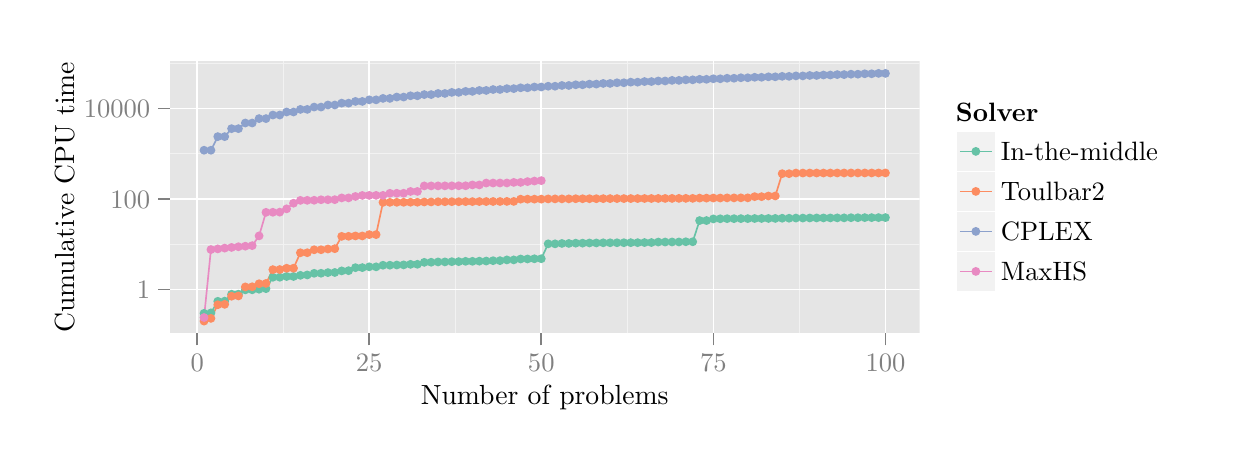
\begin{tikzpicture}[x=1pt,y=1pt]
\definecolor[named]{fillColor}{rgb}{1.00,1.00,1.00}
\path[use as bounding box,fill=fillColor,fill opacity=0.00] (0,0) rectangle (433.62,144.54);
\begin{scope}
\path[clip] (  0.00,  0.00) rectangle (433.62,144.54);
\definecolor[named]{drawColor}{rgb}{1.00,1.00,1.00}
\definecolor[named]{fillColor}{rgb}{1.00,1.00,1.00}

\path[draw=drawColor,line width= 0.6pt,line join=round,line cap=round,fill=fillColor] (  0.00,  0.00) rectangle (433.62,144.54);
\end{scope}
\begin{scope}
\path[clip] ( 51.42, 34.03) rectangle (322.26,132.50);
\definecolor[named]{fillColor}{rgb}{0.90,0.90,0.90}

\path[fill=fillColor] ( 51.42, 34.03) rectangle (322.26,132.50);
\definecolor[named]{drawColor}{rgb}{0.95,0.95,0.95}

\path[draw=drawColor,line width= 0.3pt,line join=round] ( 51.42, 66.28) --
	(322.26, 66.28);

\path[draw=drawColor,line width= 0.3pt,line join=round] ( 51.42, 98.96) --
	(322.26, 98.96);

\path[draw=drawColor,line width= 0.3pt,line join=round] ( 51.42,131.64) --
	(322.26,131.64);

\path[draw=drawColor,line width= 0.3pt,line join=round] ( 92.33, 34.03) --
	( 92.33,132.50);

\path[draw=drawColor,line width= 0.3pt,line join=round] (154.51, 34.03) --
	(154.51,132.50);

\path[draw=drawColor,line width= 0.3pt,line join=round] (216.68, 34.03) --
	(216.68,132.50);

\path[draw=drawColor,line width= 0.3pt,line join=round] (278.86, 34.03) --
	(278.86,132.50);
\definecolor[named]{drawColor}{rgb}{1.00,1.00,1.00}

\path[draw=drawColor,line width= 0.6pt,line join=round] ( 51.42, 49.93) --
	(322.26, 49.93);

\path[draw=drawColor,line width= 0.6pt,line join=round] ( 51.42, 82.62) --
	(322.26, 82.62);

\path[draw=drawColor,line width= 0.6pt,line join=round] ( 51.42,115.30) --
	(322.26,115.30);

\path[draw=drawColor,line width= 0.6pt,line join=round] ( 61.24, 34.03) --
	( 61.24,132.50);

\path[draw=drawColor,line width= 0.6pt,line join=round] (123.42, 34.03) --
	(123.42,132.50);

\path[draw=drawColor,line width= 0.6pt,line join=round] (185.59, 34.03) --
	(185.59,132.50);

\path[draw=drawColor,line width= 0.6pt,line join=round] (247.77, 34.03) --
	(247.77,132.50);

\path[draw=drawColor,line width= 0.6pt,line join=round] (309.95, 34.03) --
	(309.95,132.50);
\definecolor[named]{drawColor}{rgb}{0.40,0.76,0.65}

\path[draw=drawColor,line width= 0.6pt,line join=round] ( 63.73, 41.32) --
	( 66.22, 41.48) --
	( 68.70, 45.66) --
	( 71.19, 45.72) --
	( 73.68, 48.20) --
	( 76.16, 48.23) --
	( 78.65, 49.80) --
	( 81.14, 49.82) --
	( 83.62, 50.03) --
	( 86.11, 50.23) --
	( 88.60, 54.35) --
	( 91.09, 54.36) --
	( 93.57, 54.63) --
	( 96.06, 54.63) --
	( 98.55, 55.05) --
	(101.03, 55.19) --
	(103.52, 55.78) --
	(106.01, 55.80) --
	(108.49, 56.03) --
	(110.98, 56.08) --
	(113.47, 56.65) --
	(115.96, 56.73) --
	(118.44, 57.82) --
	(120.93, 57.84) --
	(123.42, 58.12) --
	(125.90, 58.12) --
	(128.39, 58.69) --
	(130.88, 58.71) --
	(133.37, 58.78) --
	(135.85, 58.82) --
	(138.34, 59.02) --
	(140.83, 59.04) --
	(143.31, 59.74) --
	(145.80, 59.78) --
	(148.29, 59.89) --
	(150.77, 59.90) --
	(153.26, 59.98) --
	(155.75, 60.00) --
	(158.24, 60.11) --
	(160.72, 60.11) --
	(163.21, 60.17) --
	(165.70, 60.21) --
	(168.18, 60.34) --
	(170.67, 60.35) --
	(173.16, 60.62) --
	(175.65, 60.63) --
	(178.13, 60.95) --
	(180.62, 60.96) --
	(183.11, 61.03) --
	(185.59, 61.05) --
	(188.08, 66.43) --
	(190.57, 66.43) --
	(193.05, 66.57) --
	(195.54, 66.57) --
	(198.03, 66.67) --
	(200.52, 66.68) --
	(203.00, 66.74) --
	(205.49, 66.75) --
	(207.98, 66.80) --
	(210.46, 66.81) --
	(212.95, 66.82) --
	(215.44, 66.83) --
	(217.92, 66.85) --
	(220.41, 66.85) --
	(222.90, 66.89) --
	(225.39, 66.90) --
	(227.87, 67.07) --
	(230.36, 67.08) --
	(232.85, 67.10) --
	(235.33, 67.10) --
	(237.82, 67.18) --
	(240.31, 67.18) --
	(242.80, 74.84) --
	(245.28, 74.84) --
	(247.77, 75.43) --
	(250.26, 75.48) --
	(252.74, 75.52) --
	(255.23, 75.52) --
	(257.72, 75.54) --
	(260.20, 75.54) --
	(262.69, 75.58) --
	(265.18, 75.59) --
	(267.67, 75.60) --
	(270.15, 75.61) --
	(272.64, 75.68) --
	(275.13, 75.68) --
	(277.61, 75.74) --
	(280.10, 75.74) --
	(282.59, 75.77) --
	(285.08, 75.78) --
	(287.56, 75.79) --
	(290.05, 75.79) --
	(292.54, 75.81) --
	(295.02, 75.81) --
	(297.51, 75.87) --
	(300.00, 75.87) --
	(302.48, 75.90) --
	(304.97, 75.90) --
	(307.46, 75.91) --
	(309.95, 75.91);
\definecolor[named]{drawColor}{rgb}{0.99,0.55,0.38}

\path[draw=drawColor,line width= 0.6pt,line join=round] ( 63.73, 38.51) --
	( 66.22, 39.50) --
	( 68.70, 44.42) --
	( 71.19, 44.57) --
	( 73.68, 47.50) --
	( 76.16, 47.60) --
	( 78.65, 50.86) --
	( 81.14, 50.92) --
	( 83.62, 52.01) --
	( 86.11, 52.12) --
	( 88.60, 57.11) --
	( 91.09, 57.14) --
	( 93.57, 57.61) --
	( 96.06, 57.63) --
	( 98.55, 63.21) --
	(101.03, 63.22) --
	(103.52, 64.28) --
	(106.01, 64.29) --
	(108.49, 64.56) --
	(110.98, 64.68) --
	(113.47, 69.13) --
	(115.96, 69.15) --
	(118.44, 69.28) --
	(120.93, 69.28) --
	(123.42, 69.76) --
	(125.90, 69.76) --
	(128.39, 81.42) --
	(130.88, 81.42) --
	(133.37, 81.44) --
	(135.85, 81.44) --
	(138.34, 81.46) --
	(140.83, 81.46) --
	(143.31, 81.56) --
	(145.80, 81.57) --
	(148.29, 81.64) --
	(150.77, 81.64) --
	(153.26, 81.66) --
	(155.75, 81.66) --
	(158.24, 81.69) --
	(160.72, 81.69) --
	(163.21, 81.71) --
	(165.70, 81.71) --
	(168.18, 81.73) --
	(170.67, 81.73) --
	(173.16, 81.76) --
	(175.65, 81.76) --
	(178.13, 82.57) --
	(180.62, 82.57) --
	(183.11, 82.58) --
	(185.59, 82.58) --
	(188.08, 82.66) --
	(190.57, 82.67) --
	(193.05, 82.68) --
	(195.54, 82.68) --
	(198.03, 82.73) --
	(200.52, 82.73) --
	(203.00, 82.74) --
	(205.49, 82.74) --
	(207.98, 82.76) --
	(210.46, 82.77) --
	(212.95, 82.78) --
	(215.44, 82.78) --
	(217.92, 82.79) --
	(220.41, 82.79) --
	(222.90, 82.81) --
	(225.39, 82.81) --
	(227.87, 82.83) --
	(230.36, 82.83) --
	(232.85, 82.84) --
	(235.33, 82.85) --
	(237.82, 82.86) --
	(240.31, 82.86) --
	(242.80, 82.95) --
	(245.28, 82.95) --
	(247.77, 82.98) --
	(250.26, 82.98) --
	(252.74, 83.03) --
	(255.23, 83.03) --
	(257.72, 83.05) --
	(260.20, 83.05) --
	(262.69, 83.48) --
	(265.18, 83.48) --
	(267.67, 83.71) --
	(270.15, 83.72) --
	(272.64, 91.78) --
	(275.13, 91.78) --
	(277.61, 92.01) --
	(280.10, 92.01) --
	(282.59, 92.02) --
	(285.08, 92.02) --
	(287.56, 92.02) --
	(290.05, 92.02) --
	(292.54, 92.03) --
	(295.02, 92.03) --
	(297.51, 92.04) --
	(300.00, 92.04) --
	(302.48, 92.04) --
	(304.97, 92.04) --
	(307.46, 92.04) --
	(309.95, 92.04);
\definecolor[named]{drawColor}{rgb}{0.55,0.63,0.80}

\path[draw=drawColor,line width= 0.6pt,line join=round] ( 63.73,100.25) --
	( 66.22,100.25) --
	( 68.70,105.17) --
	( 71.19,105.17) --
	( 73.68,108.05) --
	( 76.16,108.05) --
	( 78.65,110.09) --
	( 81.14,110.09) --
	( 83.62,111.68) --
	( 86.11,111.68) --
	( 88.60,112.97) --
	( 91.09,112.97) --
	( 93.57,114.07) --
	( 96.06,114.07) --
	( 98.55,115.01) --
	(101.03,115.01) --
	(103.52,115.85) --
	(106.01,115.85) --
	(108.49,116.60) --
	(110.98,116.60) --
	(113.47,117.27) --
	(115.96,117.27) --
	(118.44,117.89) --
	(120.93,117.89) --
	(123.42,118.46) --
	(125.90,118.46) --
	(128.39,118.98) --
	(130.88,118.98) --
	(133.37,119.47) --
	(135.85,119.47) --
	(138.34,119.93) --
	(140.83,119.93) --
	(143.31,120.36) --
	(145.80,120.36) --
	(148.29,120.77) --
	(150.77,120.77) --
	(153.26,121.15) --
	(155.75,121.15) --
	(158.24,121.52) --
	(160.72,121.52) --
	(163.21,121.86) --
	(165.70,121.86) --
	(168.18,122.19) --
	(170.67,122.19) --
	(173.16,122.51) --
	(175.65,122.51) --
	(178.13,122.81) --
	(180.62,122.81) --
	(183.11,123.10) --
	(185.59,123.10) --
	(188.08,123.38) --
	(190.57,123.38) --
	(193.05,123.65) --
	(195.54,123.65) --
	(198.03,123.90) --
	(200.52,123.90) --
	(203.00,124.15) --
	(205.49,124.15) --
	(207.98,124.39) --
	(210.46,124.39) --
	(212.95,124.63) --
	(215.44,124.63) --
	(217.92,124.85) --
	(220.41,124.85) --
	(222.90,125.07) --
	(225.39,125.07) --
	(227.87,125.28) --
	(230.36,125.28) --
	(232.85,125.49) --
	(235.33,125.49) --
	(237.82,125.69) --
	(240.31,125.69) --
	(242.80,125.88) --
	(245.28,125.88) --
	(247.77,126.07) --
	(250.26,126.07) --
	(252.74,126.26) --
	(255.23,126.26) --
	(257.72,126.44) --
	(260.20,126.44) --
	(262.69,126.61) --
	(265.18,126.61) --
	(267.67,126.78) --
	(270.15,126.78) --
	(272.64,126.95) --
	(275.13,126.95) --
	(277.61,127.11) --
	(280.10,127.11) --
	(282.59,127.27) --
	(285.08,127.27) --
	(287.56,127.43) --
	(290.05,127.43) --
	(292.54,127.58) --
	(295.02,127.58) --
	(297.51,127.73) --
	(300.00,127.73) --
	(302.48,127.88) --
	(304.97,127.88) --
	(307.46,128.02) --
	(309.95,128.02);
\definecolor[named]{drawColor}{rgb}{0.91,0.54,0.76}

\path[draw=drawColor,line width= 0.6pt,line join=round] ( 63.73, 39.80) --
	( 66.22, 64.36) --
	( 68.70, 64.60) --
	( 71.19, 64.88) --
	( 73.68, 65.13) --
	( 76.16, 65.38) --
	( 78.65, 65.58) --
	( 81.14, 65.78) --
	( 83.62, 69.30) --
	( 86.11, 77.81) --
	( 88.60, 77.84) --
	( 91.09, 77.88) --
	( 93.57, 79.07) --
	( 96.06, 81.11) --
	( 98.55, 82.13) --
	(101.03, 82.15) --
	(103.52, 82.18) --
	(106.01, 82.36) --
	(108.49, 82.37) --
	(110.98, 82.39) --
	(113.47, 83.02) --
	(115.96, 83.03) --
	(118.44, 83.55) --
	(120.93, 83.91) --
	(123.42, 83.93) --
	(125.90, 83.94) --
	(128.39, 83.95) --
	(130.88, 84.69) --
	(133.37, 84.71) --
	(135.85, 84.72) --
	(138.34, 85.35) --
	(140.83, 85.36) --
	(143.31, 87.36) --
	(145.80, 87.36) --
	(148.29, 87.37) --
	(150.77, 87.38) --
	(153.26, 87.39) --
	(155.75, 87.41) --
	(158.24, 87.41) --
	(160.72, 87.71) --
	(163.21, 87.71) --
	(165.70, 88.39) --
	(168.18, 88.40) --
	(170.67, 88.41) --
	(173.16, 88.42) --
	(175.65, 88.63) --
	(178.13, 88.63) --
	(180.62, 88.92) --
	(183.11, 89.12) --
	(185.59, 89.27);
\definecolor[named]{fillColor}{rgb}{0.40,0.76,0.65}

\path[fill=fillColor] ( 63.73, 41.32) circle (  1.60);

\path[fill=fillColor] ( 66.22, 41.48) circle (  1.60);

\path[fill=fillColor] ( 68.70, 45.66) circle (  1.60);

\path[fill=fillColor] ( 71.19, 45.72) circle (  1.60);

\path[fill=fillColor] ( 73.68, 48.20) circle (  1.60);

\path[fill=fillColor] ( 76.16, 48.23) circle (  1.60);

\path[fill=fillColor] ( 78.65, 49.80) circle (  1.60);

\path[fill=fillColor] ( 81.14, 49.82) circle (  1.60);

\path[fill=fillColor] ( 83.62, 50.03) circle (  1.60);

\path[fill=fillColor] ( 86.11, 50.23) circle (  1.60);

\path[fill=fillColor] ( 88.60, 54.35) circle (  1.60);

\path[fill=fillColor] ( 91.09, 54.36) circle (  1.60);

\path[fill=fillColor] ( 93.57, 54.63) circle (  1.60);

\path[fill=fillColor] ( 96.06, 54.63) circle (  1.60);

\path[fill=fillColor] ( 98.55, 55.05) circle (  1.60);

\path[fill=fillColor] (101.03, 55.19) circle (  1.60);

\path[fill=fillColor] (103.52, 55.78) circle (  1.60);

\path[fill=fillColor] (106.01, 55.80) circle (  1.60);

\path[fill=fillColor] (108.49, 56.03) circle (  1.60);

\path[fill=fillColor] (110.98, 56.08) circle (  1.60);

\path[fill=fillColor] (113.47, 56.65) circle (  1.60);

\path[fill=fillColor] (115.96, 56.73) circle (  1.60);

\path[fill=fillColor] (118.44, 57.82) circle (  1.60);

\path[fill=fillColor] (120.93, 57.84) circle (  1.60);

\path[fill=fillColor] (123.42, 58.12) circle (  1.60);

\path[fill=fillColor] (125.90, 58.12) circle (  1.60);

\path[fill=fillColor] (128.39, 58.69) circle (  1.60);

\path[fill=fillColor] (130.88, 58.71) circle (  1.60);

\path[fill=fillColor] (133.37, 58.78) circle (  1.60);

\path[fill=fillColor] (135.85, 58.82) circle (  1.60);

\path[fill=fillColor] (138.34, 59.02) circle (  1.60);

\path[fill=fillColor] (140.83, 59.04) circle (  1.60);

\path[fill=fillColor] (143.31, 59.74) circle (  1.60);

\path[fill=fillColor] (145.80, 59.78) circle (  1.60);

\path[fill=fillColor] (148.29, 59.89) circle (  1.60);

\path[fill=fillColor] (150.77, 59.90) circle (  1.60);

\path[fill=fillColor] (153.26, 59.98) circle (  1.60);

\path[fill=fillColor] (155.75, 60.00) circle (  1.60);

\path[fill=fillColor] (158.24, 60.11) circle (  1.60);

\path[fill=fillColor] (160.72, 60.11) circle (  1.60);

\path[fill=fillColor] (163.21, 60.17) circle (  1.60);

\path[fill=fillColor] (165.70, 60.21) circle (  1.60);

\path[fill=fillColor] (168.18, 60.34) circle (  1.60);

\path[fill=fillColor] (170.67, 60.35) circle (  1.60);

\path[fill=fillColor] (173.16, 60.62) circle (  1.60);

\path[fill=fillColor] (175.65, 60.63) circle (  1.60);

\path[fill=fillColor] (178.13, 60.95) circle (  1.60);

\path[fill=fillColor] (180.62, 60.96) circle (  1.60);

\path[fill=fillColor] (183.11, 61.03) circle (  1.60);

\path[fill=fillColor] (185.59, 61.05) circle (  1.60);

\path[fill=fillColor] (188.08, 66.43) circle (  1.60);

\path[fill=fillColor] (190.57, 66.43) circle (  1.60);

\path[fill=fillColor] (193.05, 66.57) circle (  1.60);

\path[fill=fillColor] (195.54, 66.57) circle (  1.60);

\path[fill=fillColor] (198.03, 66.67) circle (  1.60);

\path[fill=fillColor] (200.52, 66.68) circle (  1.60);

\path[fill=fillColor] (203.00, 66.74) circle (  1.60);

\path[fill=fillColor] (205.49, 66.75) circle (  1.60);

\path[fill=fillColor] (207.98, 66.80) circle (  1.60);

\path[fill=fillColor] (210.46, 66.81) circle (  1.60);

\path[fill=fillColor] (212.95, 66.82) circle (  1.60);

\path[fill=fillColor] (215.44, 66.83) circle (  1.60);

\path[fill=fillColor] (217.92, 66.85) circle (  1.60);

\path[fill=fillColor] (220.41, 66.85) circle (  1.60);

\path[fill=fillColor] (222.90, 66.89) circle (  1.60);

\path[fill=fillColor] (225.39, 66.90) circle (  1.60);

\path[fill=fillColor] (227.87, 67.07) circle (  1.60);

\path[fill=fillColor] (230.36, 67.08) circle (  1.60);

\path[fill=fillColor] (232.85, 67.10) circle (  1.60);

\path[fill=fillColor] (235.33, 67.10) circle (  1.60);

\path[fill=fillColor] (237.82, 67.18) circle (  1.60);

\path[fill=fillColor] (240.31, 67.18) circle (  1.60);

\path[fill=fillColor] (242.80, 74.84) circle (  1.60);

\path[fill=fillColor] (245.28, 74.84) circle (  1.60);

\path[fill=fillColor] (247.77, 75.43) circle (  1.60);

\path[fill=fillColor] (250.26, 75.48) circle (  1.60);

\path[fill=fillColor] (252.74, 75.52) circle (  1.60);

\path[fill=fillColor] (255.23, 75.52) circle (  1.60);

\path[fill=fillColor] (257.72, 75.54) circle (  1.60);

\path[fill=fillColor] (260.20, 75.54) circle (  1.60);

\path[fill=fillColor] (262.69, 75.58) circle (  1.60);

\path[fill=fillColor] (265.18, 75.59) circle (  1.60);

\path[fill=fillColor] (267.67, 75.60) circle (  1.60);

\path[fill=fillColor] (270.15, 75.61) circle (  1.60);

\path[fill=fillColor] (272.64, 75.68) circle (  1.60);

\path[fill=fillColor] (275.13, 75.68) circle (  1.60);

\path[fill=fillColor] (277.61, 75.74) circle (  1.60);

\path[fill=fillColor] (280.10, 75.74) circle (  1.60);

\path[fill=fillColor] (282.59, 75.77) circle (  1.60);

\path[fill=fillColor] (285.08, 75.78) circle (  1.60);

\path[fill=fillColor] (287.56, 75.79) circle (  1.60);

\path[fill=fillColor] (290.05, 75.79) circle (  1.60);

\path[fill=fillColor] (292.54, 75.81) circle (  1.60);

\path[fill=fillColor] (295.02, 75.81) circle (  1.60);

\path[fill=fillColor] (297.51, 75.87) circle (  1.60);

\path[fill=fillColor] (300.00, 75.87) circle (  1.60);

\path[fill=fillColor] (302.48, 75.90) circle (  1.60);

\path[fill=fillColor] (304.97, 75.90) circle (  1.60);

\path[fill=fillColor] (307.46, 75.91) circle (  1.60);

\path[fill=fillColor] (309.95, 75.91) circle (  1.60);
\definecolor[named]{fillColor}{rgb}{0.99,0.55,0.38}

\path[fill=fillColor] ( 63.73, 38.51) circle (  1.60);

\path[fill=fillColor] ( 66.22, 39.50) circle (  1.60);

\path[fill=fillColor] ( 68.70, 44.42) circle (  1.60);

\path[fill=fillColor] ( 71.19, 44.57) circle (  1.60);

\path[fill=fillColor] ( 73.68, 47.50) circle (  1.60);

\path[fill=fillColor] ( 76.16, 47.60) circle (  1.60);

\path[fill=fillColor] ( 78.65, 50.86) circle (  1.60);

\path[fill=fillColor] ( 81.14, 50.92) circle (  1.60);

\path[fill=fillColor] ( 83.62, 52.01) circle (  1.60);

\path[fill=fillColor] ( 86.11, 52.12) circle (  1.60);

\path[fill=fillColor] ( 88.60, 57.11) circle (  1.60);

\path[fill=fillColor] ( 91.09, 57.14) circle (  1.60);

\path[fill=fillColor] ( 93.57, 57.61) circle (  1.60);

\path[fill=fillColor] ( 96.06, 57.63) circle (  1.60);

\path[fill=fillColor] ( 98.55, 63.21) circle (  1.60);

\path[fill=fillColor] (101.03, 63.22) circle (  1.60);

\path[fill=fillColor] (103.52, 64.28) circle (  1.60);

\path[fill=fillColor] (106.01, 64.29) circle (  1.60);

\path[fill=fillColor] (108.49, 64.56) circle (  1.60);

\path[fill=fillColor] (110.98, 64.68) circle (  1.60);

\path[fill=fillColor] (113.47, 69.13) circle (  1.60);

\path[fill=fillColor] (115.96, 69.15) circle (  1.60);

\path[fill=fillColor] (118.44, 69.28) circle (  1.60);

\path[fill=fillColor] (120.93, 69.28) circle (  1.60);

\path[fill=fillColor] (123.42, 69.76) circle (  1.60);

\path[fill=fillColor] (125.90, 69.76) circle (  1.60);

\path[fill=fillColor] (128.39, 81.42) circle (  1.60);

\path[fill=fillColor] (130.88, 81.42) circle (  1.60);

\path[fill=fillColor] (133.37, 81.44) circle (  1.60);

\path[fill=fillColor] (135.85, 81.44) circle (  1.60);

\path[fill=fillColor] (138.34, 81.46) circle (  1.60);

\path[fill=fillColor] (140.83, 81.46) circle (  1.60);

\path[fill=fillColor] (143.31, 81.56) circle (  1.60);

\path[fill=fillColor] (145.80, 81.57) circle (  1.60);

\path[fill=fillColor] (148.29, 81.64) circle (  1.60);

\path[fill=fillColor] (150.77, 81.64) circle (  1.60);

\path[fill=fillColor] (153.26, 81.66) circle (  1.60);

\path[fill=fillColor] (155.75, 81.66) circle (  1.60);

\path[fill=fillColor] (158.24, 81.69) circle (  1.60);

\path[fill=fillColor] (160.72, 81.69) circle (  1.60);

\path[fill=fillColor] (163.21, 81.71) circle (  1.60);

\path[fill=fillColor] (165.70, 81.71) circle (  1.60);

\path[fill=fillColor] (168.18, 81.73) circle (  1.60);

\path[fill=fillColor] (170.67, 81.73) circle (  1.60);

\path[fill=fillColor] (173.16, 81.76) circle (  1.60);

\path[fill=fillColor] (175.65, 81.76) circle (  1.60);

\path[fill=fillColor] (178.13, 82.57) circle (  1.60);

\path[fill=fillColor] (180.62, 82.57) circle (  1.60);

\path[fill=fillColor] (183.11, 82.58) circle (  1.60);

\path[fill=fillColor] (185.59, 82.58) circle (  1.60);

\path[fill=fillColor] (188.08, 82.66) circle (  1.60);

\path[fill=fillColor] (190.57, 82.67) circle (  1.60);

\path[fill=fillColor] (193.05, 82.68) circle (  1.60);

\path[fill=fillColor] (195.54, 82.68) circle (  1.60);

\path[fill=fillColor] (198.03, 82.73) circle (  1.60);

\path[fill=fillColor] (200.52, 82.73) circle (  1.60);

\path[fill=fillColor] (203.00, 82.74) circle (  1.60);

\path[fill=fillColor] (205.49, 82.74) circle (  1.60);

\path[fill=fillColor] (207.98, 82.76) circle (  1.60);

\path[fill=fillColor] (210.46, 82.77) circle (  1.60);

\path[fill=fillColor] (212.95, 82.78) circle (  1.60);

\path[fill=fillColor] (215.44, 82.78) circle (  1.60);

\path[fill=fillColor] (217.92, 82.79) circle (  1.60);

\path[fill=fillColor] (220.41, 82.79) circle (  1.60);

\path[fill=fillColor] (222.90, 82.81) circle (  1.60);

\path[fill=fillColor] (225.39, 82.81) circle (  1.60);

\path[fill=fillColor] (227.87, 82.83) circle (  1.60);

\path[fill=fillColor] (230.36, 82.83) circle (  1.60);

\path[fill=fillColor] (232.85, 82.84) circle (  1.60);

\path[fill=fillColor] (235.33, 82.85) circle (  1.60);

\path[fill=fillColor] (237.82, 82.86) circle (  1.60);

\path[fill=fillColor] (240.31, 82.86) circle (  1.60);

\path[fill=fillColor] (242.80, 82.95) circle (  1.60);

\path[fill=fillColor] (245.28, 82.95) circle (  1.60);

\path[fill=fillColor] (247.77, 82.98) circle (  1.60);

\path[fill=fillColor] (250.26, 82.98) circle (  1.60);

\path[fill=fillColor] (252.74, 83.03) circle (  1.60);

\path[fill=fillColor] (255.23, 83.03) circle (  1.60);

\path[fill=fillColor] (257.72, 83.05) circle (  1.60);

\path[fill=fillColor] (260.20, 83.05) circle (  1.60);

\path[fill=fillColor] (262.69, 83.48) circle (  1.60);

\path[fill=fillColor] (265.18, 83.48) circle (  1.60);

\path[fill=fillColor] (267.67, 83.71) circle (  1.60);

\path[fill=fillColor] (270.15, 83.72) circle (  1.60);

\path[fill=fillColor] (272.64, 91.78) circle (  1.60);

\path[fill=fillColor] (275.13, 91.78) circle (  1.60);

\path[fill=fillColor] (277.61, 92.01) circle (  1.60);

\path[fill=fillColor] (280.10, 92.01) circle (  1.60);

\path[fill=fillColor] (282.59, 92.02) circle (  1.60);

\path[fill=fillColor] (285.08, 92.02) circle (  1.60);

\path[fill=fillColor] (287.56, 92.02) circle (  1.60);

\path[fill=fillColor] (290.05, 92.02) circle (  1.60);

\path[fill=fillColor] (292.54, 92.03) circle (  1.60);

\path[fill=fillColor] (295.02, 92.03) circle (  1.60);

\path[fill=fillColor] (297.51, 92.04) circle (  1.60);

\path[fill=fillColor] (300.00, 92.04) circle (  1.60);

\path[fill=fillColor] (302.48, 92.04) circle (  1.60);

\path[fill=fillColor] (304.97, 92.04) circle (  1.60);

\path[fill=fillColor] (307.46, 92.04) circle (  1.60);

\path[fill=fillColor] (309.95, 92.04) circle (  1.60);
\definecolor[named]{fillColor}{rgb}{0.55,0.63,0.80}

\path[fill=fillColor] ( 63.73,100.25) circle (  1.60);

\path[fill=fillColor] ( 66.22,100.25) circle (  1.60);

\path[fill=fillColor] ( 68.70,105.17) circle (  1.60);

\path[fill=fillColor] ( 71.19,105.17) circle (  1.60);

\path[fill=fillColor] ( 73.68,108.05) circle (  1.60);

\path[fill=fillColor] ( 76.16,108.05) circle (  1.60);

\path[fill=fillColor] ( 78.65,110.09) circle (  1.60);

\path[fill=fillColor] ( 81.14,110.09) circle (  1.60);

\path[fill=fillColor] ( 83.62,111.68) circle (  1.60);

\path[fill=fillColor] ( 86.11,111.68) circle (  1.60);

\path[fill=fillColor] ( 88.60,112.97) circle (  1.60);

\path[fill=fillColor] ( 91.09,112.97) circle (  1.60);

\path[fill=fillColor] ( 93.57,114.07) circle (  1.60);

\path[fill=fillColor] ( 96.06,114.07) circle (  1.60);

\path[fill=fillColor] ( 98.55,115.01) circle (  1.60);

\path[fill=fillColor] (101.03,115.01) circle (  1.60);

\path[fill=fillColor] (103.52,115.85) circle (  1.60);

\path[fill=fillColor] (106.01,115.85) circle (  1.60);

\path[fill=fillColor] (108.49,116.60) circle (  1.60);

\path[fill=fillColor] (110.98,116.60) circle (  1.60);

\path[fill=fillColor] (113.47,117.27) circle (  1.60);

\path[fill=fillColor] (115.96,117.27) circle (  1.60);

\path[fill=fillColor] (118.44,117.89) circle (  1.60);

\path[fill=fillColor] (120.93,117.89) circle (  1.60);

\path[fill=fillColor] (123.42,118.46) circle (  1.60);

\path[fill=fillColor] (125.90,118.46) circle (  1.60);

\path[fill=fillColor] (128.39,118.98) circle (  1.60);

\path[fill=fillColor] (130.88,118.98) circle (  1.60);

\path[fill=fillColor] (133.37,119.47) circle (  1.60);

\path[fill=fillColor] (135.85,119.47) circle (  1.60);

\path[fill=fillColor] (138.34,119.93) circle (  1.60);

\path[fill=fillColor] (140.83,119.93) circle (  1.60);

\path[fill=fillColor] (143.31,120.36) circle (  1.60);

\path[fill=fillColor] (145.80,120.36) circle (  1.60);

\path[fill=fillColor] (148.29,120.77) circle (  1.60);

\path[fill=fillColor] (150.77,120.77) circle (  1.60);

\path[fill=fillColor] (153.26,121.15) circle (  1.60);

\path[fill=fillColor] (155.75,121.15) circle (  1.60);

\path[fill=fillColor] (158.24,121.52) circle (  1.60);

\path[fill=fillColor] (160.72,121.52) circle (  1.60);

\path[fill=fillColor] (163.21,121.86) circle (  1.60);

\path[fill=fillColor] (165.70,121.86) circle (  1.60);

\path[fill=fillColor] (168.18,122.19) circle (  1.60);

\path[fill=fillColor] (170.67,122.19) circle (  1.60);

\path[fill=fillColor] (173.16,122.51) circle (  1.60);

\path[fill=fillColor] (175.65,122.51) circle (  1.60);

\path[fill=fillColor] (178.13,122.81) circle (  1.60);

\path[fill=fillColor] (180.62,122.81) circle (  1.60);

\path[fill=fillColor] (183.11,123.10) circle (  1.60);

\path[fill=fillColor] (185.59,123.10) circle (  1.60);

\path[fill=fillColor] (188.08,123.38) circle (  1.60);

\path[fill=fillColor] (190.57,123.38) circle (  1.60);

\path[fill=fillColor] (193.05,123.65) circle (  1.60);

\path[fill=fillColor] (195.54,123.65) circle (  1.60);

\path[fill=fillColor] (198.03,123.90) circle (  1.60);

\path[fill=fillColor] (200.52,123.90) circle (  1.60);

\path[fill=fillColor] (203.00,124.15) circle (  1.60);

\path[fill=fillColor] (205.49,124.15) circle (  1.60);

\path[fill=fillColor] (207.98,124.39) circle (  1.60);

\path[fill=fillColor] (210.46,124.39) circle (  1.60);

\path[fill=fillColor] (212.95,124.63) circle (  1.60);

\path[fill=fillColor] (215.44,124.63) circle (  1.60);

\path[fill=fillColor] (217.92,124.85) circle (  1.60);

\path[fill=fillColor] (220.41,124.85) circle (  1.60);

\path[fill=fillColor] (222.90,125.07) circle (  1.60);

\path[fill=fillColor] (225.39,125.07) circle (  1.60);

\path[fill=fillColor] (227.87,125.28) circle (  1.60);

\path[fill=fillColor] (230.36,125.28) circle (  1.60);

\path[fill=fillColor] (232.85,125.49) circle (  1.60);

\path[fill=fillColor] (235.33,125.49) circle (  1.60);

\path[fill=fillColor] (237.82,125.69) circle (  1.60);

\path[fill=fillColor] (240.31,125.69) circle (  1.60);

\path[fill=fillColor] (242.80,125.88) circle (  1.60);

\path[fill=fillColor] (245.28,125.88) circle (  1.60);

\path[fill=fillColor] (247.77,126.07) circle (  1.60);

\path[fill=fillColor] (250.26,126.07) circle (  1.60);

\path[fill=fillColor] (252.74,126.26) circle (  1.60);

\path[fill=fillColor] (255.23,126.26) circle (  1.60);

\path[fill=fillColor] (257.72,126.44) circle (  1.60);

\path[fill=fillColor] (260.20,126.44) circle (  1.60);

\path[fill=fillColor] (262.69,126.61) circle (  1.60);

\path[fill=fillColor] (265.18,126.61) circle (  1.60);

\path[fill=fillColor] (267.67,126.78) circle (  1.60);

\path[fill=fillColor] (270.15,126.78) circle (  1.60);

\path[fill=fillColor] (272.64,126.95) circle (  1.60);

\path[fill=fillColor] (275.13,126.95) circle (  1.60);

\path[fill=fillColor] (277.61,127.11) circle (  1.60);

\path[fill=fillColor] (280.10,127.11) circle (  1.60);

\path[fill=fillColor] (282.59,127.27) circle (  1.60);

\path[fill=fillColor] (285.08,127.27) circle (  1.60);

\path[fill=fillColor] (287.56,127.43) circle (  1.60);

\path[fill=fillColor] (290.05,127.43) circle (  1.60);

\path[fill=fillColor] (292.54,127.58) circle (  1.60);

\path[fill=fillColor] (295.02,127.58) circle (  1.60);

\path[fill=fillColor] (297.51,127.73) circle (  1.60);

\path[fill=fillColor] (300.00,127.73) circle (  1.60);

\path[fill=fillColor] (302.48,127.88) circle (  1.60);

\path[fill=fillColor] (304.97,127.88) circle (  1.60);

\path[fill=fillColor] (307.46,128.02) circle (  1.60);

\path[fill=fillColor] (309.95,128.02) circle (  1.60);
\definecolor[named]{fillColor}{rgb}{0.91,0.54,0.76}

\path[fill=fillColor] ( 63.73, 39.80) circle (  1.60);

\path[fill=fillColor] ( 66.22, 64.36) circle (  1.60);

\path[fill=fillColor] ( 68.70, 64.60) circle (  1.60);

\path[fill=fillColor] ( 71.19, 64.88) circle (  1.60);

\path[fill=fillColor] ( 73.68, 65.13) circle (  1.60);

\path[fill=fillColor] ( 76.16, 65.38) circle (  1.60);

\path[fill=fillColor] ( 78.65, 65.58) circle (  1.60);

\path[fill=fillColor] ( 81.14, 65.78) circle (  1.60);

\path[fill=fillColor] ( 83.62, 69.30) circle (  1.60);

\path[fill=fillColor] ( 86.11, 77.81) circle (  1.60);

\path[fill=fillColor] ( 88.60, 77.84) circle (  1.60);

\path[fill=fillColor] ( 91.09, 77.88) circle (  1.60);

\path[fill=fillColor] ( 93.57, 79.07) circle (  1.60);

\path[fill=fillColor] ( 96.06, 81.11) circle (  1.60);

\path[fill=fillColor] ( 98.55, 82.13) circle (  1.60);

\path[fill=fillColor] (101.03, 82.15) circle (  1.60);

\path[fill=fillColor] (103.52, 82.18) circle (  1.60);

\path[fill=fillColor] (106.01, 82.36) circle (  1.60);

\path[fill=fillColor] (108.49, 82.37) circle (  1.60);

\path[fill=fillColor] (110.98, 82.39) circle (  1.60);

\path[fill=fillColor] (113.47, 83.02) circle (  1.60);

\path[fill=fillColor] (115.96, 83.03) circle (  1.60);

\path[fill=fillColor] (118.44, 83.55) circle (  1.60);

\path[fill=fillColor] (120.93, 83.91) circle (  1.60);

\path[fill=fillColor] (123.42, 83.93) circle (  1.60);

\path[fill=fillColor] (125.90, 83.94) circle (  1.60);

\path[fill=fillColor] (128.39, 83.95) circle (  1.60);

\path[fill=fillColor] (130.88, 84.69) circle (  1.60);

\path[fill=fillColor] (133.37, 84.71) circle (  1.60);

\path[fill=fillColor] (135.85, 84.72) circle (  1.60);

\path[fill=fillColor] (138.34, 85.35) circle (  1.60);

\path[fill=fillColor] (140.83, 85.36) circle (  1.60);

\path[fill=fillColor] (143.31, 87.36) circle (  1.60);

\path[fill=fillColor] (145.80, 87.36) circle (  1.60);

\path[fill=fillColor] (148.29, 87.37) circle (  1.60);

\path[fill=fillColor] (150.77, 87.38) circle (  1.60);

\path[fill=fillColor] (153.26, 87.39) circle (  1.60);

\path[fill=fillColor] (155.75, 87.41) circle (  1.60);

\path[fill=fillColor] (158.24, 87.41) circle (  1.60);

\path[fill=fillColor] (160.72, 87.71) circle (  1.60);

\path[fill=fillColor] (163.21, 87.71) circle (  1.60);

\path[fill=fillColor] (165.70, 88.39) circle (  1.60);

\path[fill=fillColor] (168.18, 88.40) circle (  1.60);

\path[fill=fillColor] (170.67, 88.41) circle (  1.60);

\path[fill=fillColor] (173.16, 88.42) circle (  1.60);

\path[fill=fillColor] (175.65, 88.63) circle (  1.60);

\path[fill=fillColor] (178.13, 88.63) circle (  1.60);

\path[fill=fillColor] (180.62, 88.92) circle (  1.60);

\path[fill=fillColor] (183.11, 89.12) circle (  1.60);

\path[fill=fillColor] (185.59, 89.27) circle (  1.60);
\end{scope}
\begin{scope}
\path[clip] (  0.00,  0.00) rectangle (433.62,144.54);
\definecolor[named]{drawColor}{rgb}{0.50,0.50,0.50}

\node[text=drawColor,anchor=base east,inner sep=0pt, outer sep=0pt, scale=  0.96] at ( 44.30, 46.63) {1};

\node[text=drawColor,anchor=base east,inner sep=0pt, outer sep=0pt, scale=  0.96] at ( 44.30, 79.31) {100};

\node[text=drawColor,anchor=base east,inner sep=0pt, outer sep=0pt, scale=  0.96] at ( 44.30,112.00) {10000};
\end{scope}
\begin{scope}
\path[clip] (  0.00,  0.00) rectangle (433.62,144.54);
\definecolor[named]{drawColor}{rgb}{0.50,0.50,0.50}

\path[draw=drawColor,line width= 0.6pt,line join=round] ( 47.15, 49.93) --
	( 51.42, 49.93);

\path[draw=drawColor,line width= 0.6pt,line join=round] ( 47.15, 82.62) --
	( 51.42, 82.62);

\path[draw=drawColor,line width= 0.6pt,line join=round] ( 47.15,115.30) --
	( 51.42,115.30);
\end{scope}
\begin{scope}
\path[clip] (  0.00,  0.00) rectangle (433.62,144.54);
\definecolor[named]{drawColor}{rgb}{0.50,0.50,0.50}

\path[draw=drawColor,line width= 0.6pt,line join=round] ( 61.24, 29.77) --
	( 61.24, 34.03);

\path[draw=drawColor,line width= 0.6pt,line join=round] (123.42, 29.77) --
	(123.42, 34.03);

\path[draw=drawColor,line width= 0.6pt,line join=round] (185.59, 29.77) --
	(185.59, 34.03);

\path[draw=drawColor,line width= 0.6pt,line join=round] (247.77, 29.77) --
	(247.77, 34.03);

\path[draw=drawColor,line width= 0.6pt,line join=round] (309.95, 29.77) --
	(309.95, 34.03);
\end{scope}
\begin{scope}
\path[clip] (  0.00,  0.00) rectangle (433.62,144.54);
\definecolor[named]{drawColor}{rgb}{0.50,0.50,0.50}

\node[text=drawColor,anchor=base,inner sep=0pt, outer sep=0pt, scale=  0.96] at ( 61.24, 20.31) {0};

\node[text=drawColor,anchor=base,inner sep=0pt, outer sep=0pt, scale=  0.96] at (123.42, 20.31) {25};

\node[text=drawColor,anchor=base,inner sep=0pt, outer sep=0pt, scale=  0.96] at (185.59, 20.31) {50};

\node[text=drawColor,anchor=base,inner sep=0pt, outer sep=0pt, scale=  0.96] at (247.77, 20.31) {75};

\node[text=drawColor,anchor=base,inner sep=0pt, outer sep=0pt, scale=  0.96] at (309.95, 20.31) {100};
\end{scope}
\begin{scope}
\path[clip] (  0.00,  0.00) rectangle (433.62,144.54);
\definecolor[named]{drawColor}{rgb}{0.00,0.00,0.00}

\node[text=drawColor,anchor=base,inner sep=0pt, outer sep=0pt, scale=  1] at (186.84,  8.53) {Number of problems};
\end{scope}
\begin{scope}
\path[clip] (  0.00,  0.00) rectangle (433.62,144.54);
\definecolor[named]{drawColor}{rgb}{0.00,0.00,0.00}

\node[text=drawColor,rotate= 90.00,anchor=base,inner sep=0pt, outer sep=0pt, scale=  1] at ( 16.80, 83.26) {Cumulative CPU time};
\end{scope}
\begin{scope}
\path[clip] (  0.00,  0.00) rectangle (433.62,144.54);
\definecolor[named]{fillColor}{rgb}{1.00,1.00,1.00}

\path[fill=fillColor] (331.12, 44.97) rectangle (412.71,121.56);
\end{scope}
\begin{scope}
\path[clip] (  0.00,  0.00) rectangle (433.62,144.54);
\definecolor[named]{drawColor}{rgb}{0.00,0.00,0.00}

\node[text=drawColor,anchor=base west,inner sep=0pt, outer sep=0pt, scale=  0.96] at (335.39,110.67) {\bfseries Solver};
\end{scope}
\begin{scope}
\path[clip] (  0.00,  0.00) rectangle (433.62,144.54);
\definecolor[named]{drawColor}{rgb}{1.00,1.00,1.00}
\definecolor[named]{fillColor}{rgb}{0.95,0.95,0.95}

\path[draw=drawColor,line width= 0.6pt,line join=round,line cap=round,fill=fillColor] (335.39, 92.60) rectangle (349.85,107.05);
\end{scope}
\begin{scope}
\path[clip] (  0.00,  0.00) rectangle (433.62,144.54);
\definecolor[named]{drawColor}{rgb}{0.40,0.76,0.65}

\path[draw=drawColor,line width= 0.6pt,line join=round] (336.84, 99.83) -- (348.40, 99.83);
\end{scope}
\begin{scope}
\path[clip] (  0.00,  0.00) rectangle (433.62,144.54);
\definecolor[named]{fillColor}{rgb}{0.40,0.76,0.65}

\path[fill=fillColor] (342.62, 99.83) circle (  1.60);
\end{scope}
\begin{scope}
\path[clip] (  0.00,  0.00) rectangle (433.62,144.54);
\definecolor[named]{drawColor}{rgb}{1.00,1.00,1.00}
\definecolor[named]{fillColor}{rgb}{0.95,0.95,0.95}

\path[draw=drawColor,line width= 0.6pt,line join=round,line cap=round,fill=fillColor] (335.39, 78.15) rectangle (349.85, 92.60);
\end{scope}
\begin{scope}
\path[clip] (  0.00,  0.00) rectangle (433.62,144.54);
\definecolor[named]{drawColor}{rgb}{0.99,0.55,0.38}

\path[draw=drawColor,line width= 0.6pt,line join=round] (336.84, 85.37) -- (348.40, 85.37);
\end{scope}
\begin{scope}
\path[clip] (  0.00,  0.00) rectangle (433.62,144.54);
\definecolor[named]{fillColor}{rgb}{0.99,0.55,0.38}

\path[fill=fillColor] (342.62, 85.37) circle (  1.60);
\end{scope}
\begin{scope}
\path[clip] (  0.00,  0.00) rectangle (433.62,144.54);
\definecolor[named]{drawColor}{rgb}{1.00,1.00,1.00}
\definecolor[named]{fillColor}{rgb}{0.95,0.95,0.95}

\path[draw=drawColor,line width= 0.6pt,line join=round,line cap=round,fill=fillColor] (335.39, 63.69) rectangle (349.85, 78.15);
\end{scope}
\begin{scope}
\path[clip] (  0.00,  0.00) rectangle (433.62,144.54);
\definecolor[named]{drawColor}{rgb}{0.55,0.63,0.80}

\path[draw=drawColor,line width= 0.6pt,line join=round] (336.84, 70.92) -- (348.40, 70.92);
\end{scope}
\begin{scope}
\path[clip] (  0.00,  0.00) rectangle (433.62,144.54);
\definecolor[named]{fillColor}{rgb}{0.55,0.63,0.80}

\path[fill=fillColor] (342.62, 70.92) circle (  1.60);
\end{scope}
\begin{scope}
\path[clip] (  0.00,  0.00) rectangle (433.62,144.54);
\definecolor[named]{drawColor}{rgb}{1.00,1.00,1.00}
\definecolor[named]{fillColor}{rgb}{0.95,0.95,0.95}

\path[draw=drawColor,line width= 0.6pt,line join=round,line cap=round,fill=fillColor] (335.39, 49.24) rectangle (349.85, 63.69);
\end{scope}
\begin{scope}
\path[clip] (  0.00,  0.00) rectangle (433.62,144.54);
\definecolor[named]{drawColor}{rgb}{0.91,0.54,0.76}

\path[draw=drawColor,line width= 0.6pt,line join=round] (336.84, 56.46) -- (348.40, 56.46);
\end{scope}
\begin{scope}
\path[clip] (  0.00,  0.00) rectangle (433.62,144.54);
\definecolor[named]{fillColor}{rgb}{0.91,0.54,0.76}

\path[fill=fillColor] (342.62, 56.46) circle (  1.60);
\end{scope}
\begin{scope}
\path[clip] (  0.00,  0.00) rectangle (433.62,144.54);
\definecolor[named]{drawColor}{rgb}{0.00,0.00,0.00}

\node[text=drawColor,anchor=base west,inner sep=0pt, outer sep=0pt, scale=  0.96] at (351.65, 96.52) {In-the-middle};
\end{scope}
\begin{scope}
\path[clip] (  0.00,  0.00) rectangle (433.62,144.54);
\definecolor[named]{drawColor}{rgb}{0.00,0.00,0.00}

\node[text=drawColor,anchor=base west,inner sep=0pt, outer sep=0pt, scale=  0.96] at (351.65, 82.07) {Toulbar2};
\end{scope}
\begin{scope}
\path[clip] (  0.00,  0.00) rectangle (433.62,144.54);
\definecolor[named]{drawColor}{rgb}{0.00,0.00,0.00}

\node[text=drawColor,anchor=base west,inner sep=0pt, outer sep=0pt, scale=  0.96] at (351.65, 67.61) {CPLEX};
\end{scope}
\begin{scope}
\path[clip] (  0.00,  0.00) rectangle (433.62,144.54);
\definecolor[named]{drawColor}{rgb}{0.00,0.00,0.00}

\node[text=drawColor,anchor=base west,inner sep=0pt, outer sep=0pt, scale=  0.96] at (351.65, 53.16) {MaxHS};
\end{scope}
\end{tikzpicture}
}
	\end{figcenter}
	\caption{Accumulated runtime of the algorithms in four different sets. Note the logarithmic scale of the \(y\) axis.}
	\label{fig:cactus-std}
\end{figure}

\begin{table}
	\centering
	% Updated 2014-05-25
	\caption{
		Solved problems.
		For each problem instance used in the benchmark, the number of problems solved by each solver is listed.
		%Some problem sets have been omitted.
	}
	% [review] - should this be in an appendix?
	\label{tab:number-solved}
	\begin{figcenter}
	\begin{tabular}{xyccHccc}
		\toprule
			{} & {} & {} & \multicolumn{5}{c}{\(\#\) solved} \\
			\cmidrule(rl){4-8}
			{\normalsize Category} & {\normalsize Set} & {\(\#\) of problems} & {ITM} & {MPLP2} & {Toulbar2} & {CPLEX} & {MaxHS} \\
		\midrule
\acrshort{cfn}	&	Auction	&	170	&	102	&	97	&	170	&	170	&	170 \\
				&	CELAR	&	16	&	10	&	16	&	16	&	16	&	0 \\
				&	Pedigree	&	10	&	10	&	0	&	10	&	5	&	5 \\
				&	ProteinDesign	&	10	&	10	&	9	&	10	&	10	&	0 \\
				&	SPOT5	&	20	&	5	&	1	&	20	&	20	&	5 \\
				&	Warehouse	&	55	&	38	&	54	&	55	&	55	&	47 \\
%\acrshort{cp}	&	AMaze	&	6	&	0	&	0	&	2	&	0	&	6 \\
%				&	FastFood	&	6	&	1	&	0	&	1	&	1	&	1 \\
%\acrshort{cp}	&	Golomb	&	6	&	0	&	0	&	3	&	0	&	3 \\
\acrshort{cp}	&	OnCallRostering	&	5	&	3	&	0	&	3	&	3	&	3 \\
				&	ParityLearning	&	7	&	7	&	0	&	7	&	7	&	3 \\
%				&	VRP	&	5	&	0	&	0	&	5	&	0	&	0 \\
%\acrshort{cvpr}	&	ChineseChars	&	100	&	0	&	100	&	100	&	100	&	0 \\
%				&	ColorSeg	&	21	&	0	&	16	&	21	&	5	&	0 \\
\acrshort{cvpr}	&	GeomSurf	&	600	&	600	&	324	&	600	&	600	&	310 \\
				&	InPainting	&	4	&	4	&	4	&	4	&	3	&	0 \\
				&	Matching	&	4	&	4	&	1	&	4	&	4	&	0 \\
%				&	MatchingStereo	&	2	&	0	&	2	&	2	&	0	&	0 \\
				&	ObjectSeg	&	5	&	5	&	5	&	5	&	4	&	0 \\
%				&	PhotoMontage	&	2	&	0	&	0	&	0	&	0	&	0 \\
				&	SceneDecomp	&	715	&	715	&	715	&	715	&	715	&	1 \\
Max-\acrshort{csp}	&	BlackHole	&	37	&	37	&	0	&	37	&	37	&	10 \\
				&	Coloring	&	22	&	22	&	0	&	20	&	22	&	12 \\
				&	Composed	&	80	&	80	&	80	&	80	&	80	&	80 \\
				&	EHI	&	200	&	200	&	0	&	200	&	200	&	0 \\
				&	Geometric	&	100	&	100	&	0	&	100	&	100	&	88 \\
				&	Langford	&	4	&	4	&	1	&	4	&	4	&	2 \\
				&	QCP	&	60	&	60	&	4	&	60	&	60	&	46 \\
\acrshort{mrf}	&	DBN	&	108	&	108	&	108	&	108	&	108	&	30 \\
				&	Grid	&	21	&	0	&	21	&	21	&	21	&	4 \\
				&	ImageAlignment	&	10	&	10	&	10	&	10	&	8	&	0 \\
				&	Linkage	&	22	&	8	&	5	&	22	&	22	&	20 \\
				&	ObjectDetection	&	37	&	37	&	23	&	37	&	37	&	0 \\
				&	ProteinFolding	&	21	&	20	&	21	&	21	&	10	&	0 \\
				&	Segmentation	&	100	&	100	&	100	&	100	&	100	&	50 \\
%\acrshort{wpms}	&	Haplotyping	&	100	&	0	&	0	&	100	&	96	&	25 \\
\acrshort{wpms}	&	MaxClique	&	62	&	46	&	56	&	62	&	62	&	36 \\
%				&	MIPLib	&	12	&	0	&	0	&	5	&	5	&	3 \\
%				&	PackupWeighted	&	99	&	0	&	0	&	98	&	99	&	85 \\
%				&	PlanningWithPref	&	29	&	0	&	0	&	24	&	21	&	27 \\
%				&	TimeTabling	&	25	&	0	&	0	&	1	&	1	&	1 \\
%				&	Upgradeability	&	100	&	0	&	0	&	100	&	100	&	100 \\
		\bottomrule
	\end{tabular}
	\end{figcenter}
\end{table}
